\chapter{Pion Photoproduction}\label{sec:PionPhotoproduction}
We now consider the case of pion photoproduction. In the model mentioned in section \ref{sec:model} the nucleon is in a superposition of states with an arbitrary number of pions. However, we constrain the model to the one-pion approximation. This is illustrated in figure \ref{Multicomponent}
\begin{marginfigure}
	\centering
	

% Pattern Info

\tikzset{
	pattern size/.store in=\mcSize, 
	pattern size = 5pt,
	pattern thickness/.store in=\mcThickness, 
	pattern thickness = 0.3pt,
	pattern radius/.store in=\mcRadius, 
	pattern radius = 1pt}
\makeatletter
\pgfutil@ifundefined{pgf@pattern@name@_t53nej2q6}{
	\makeatletter
	\pgfdeclarepatternformonly[\mcRadius,\mcThickness,\mcSize]{_t53nej2q6}
	{\pgfpoint{-0.5*\mcSize}{-0.5*\mcSize}}
	{\pgfpoint{0.5*\mcSize}{0.5*\mcSize}}
	{\pgfpoint{\mcSize}{\mcSize}}
	{
		\pgfsetcolor{\tikz@pattern@color}
		\pgfsetlinewidth{\mcThickness}
		\pgfpathcircle\pgfpointorigin{\mcRadius}
		\pgfusepath{stroke}
}}
\makeatother
\tikzset{every picture/.style={line width=0.75pt}} %set default line width to 0.75pt        

\begin{tikzpicture}[x=0.75pt,y=0.75pt,yscale=-1,xscale=1]
	%uncomment if require: \path (0,389); %set diagram left start at 0, and has height of 389
	
	%Flowchart: Connector [id:dp12351893787926194] 
	\draw  [color={rgb, 255:red, 208; green, 2; blue, 27 }  ,draw opacity=1 ][pattern=_t53nej2q6,pattern size=2.925pt,pattern thickness=0.75pt,pattern radius=0.75pt, pattern color={rgb, 255:red, 208; green, 2; blue, 27}][line width=0.75]  (315.75,205) .. controls (315.75,154.6) and (356.6,113.75) .. (407,113.75) .. controls (457.4,113.75) and (498.25,154.6) .. (498.25,205) .. controls (498.25,255.4) and (457.4,296.25) .. (407,296.25) .. controls (356.6,296.25) and (315.75,255.4) .. (315.75,205) -- cycle ;
	%Flowchart: Connector [id:dp2648272257538774] 
	\draw  [color={rgb, 255:red, 0; green, 0; blue, 0 }  ,draw opacity=1 ][fill={rgb, 255:red, 126; green, 211; blue, 33 }  ,fill opacity=1 ][line width=0.75]  (379,205) .. controls (379,189.54) and (391.54,177) .. (407,177) .. controls (422.46,177) and (435,189.54) .. (435,205) .. controls (435,220.46) and (422.46,233) .. (407,233) .. controls (391.54,233) and (379,220.46) .. (379,205) -- cycle ;
	%Shape: Circle [id:dp5293194247132722] 
	\draw  [fill={rgb, 255:red, 255; green, 255; blue, 255 }  ,fill opacity=1 ] (397,151) .. controls (397,145.48) and (401.48,141) .. (407,141) .. controls (412.52,141) and (417,145.48) .. (417,151) .. controls (417,156.52) and (412.52,161) .. (407,161) .. controls (401.48,161) and (397,156.52) .. (397,151) -- cycle ;
	
	% Text Node
	\draw (400,200) node [anchor=north west][inner sep=0.75pt]  [color={rgb, 255:red, 0; green, 0; blue, 0 }  ,opacity=1 ]  {$N$};
	% Text Node
	\draw (401,147) node [anchor=north west][inner sep=0.75pt]  [color={rgb, 255:red, 0; green, 0; blue, 0 }  ,opacity=1 ]  {$\pi $};
	
	
\end{tikzpicture}
	\caption{Illustration of the dressed nucleon. In the centre (green) is a nucleon, and surrounding it is a cloud of virtual pions (red field). }
	\label{Multicomponent}
\end{marginfigure}
There are four pion photoproduction processes on nucleons, and these are given by
\begin{align}
	p \gamma & \rightarrow p \pi^0 \label{photonew1}\\
	p \gamma & \rightarrow n \pi^+ \label{photonew2}\\
	n \gamma & \rightarrow n \pi^0 \label{photonew3}\\
	n \gamma & \rightarrow p \pi^- \label{photonew4}.
\end{align}
Within the framework of this model, we would anticipate these processes by applying equation \eqref{isocoeff} to the isospin state of the given nucleon, i.e.
\begin{equation} \label{isovectorex}
	(\vec{\tau}\cdot\vec{\pi}) p = p\pi^0 + \sqrt{2}n\pi^+,
\end{equation}
for the isospin state of the proton and similarly for the neutron. As mentioned in section \ref{sec:DressingofProton}, the pion is trapped behind a potential barrier of height $140$ MeV and cannot leave unless an incoming photon of sufficient energy hits the pion-nucleon system and photodisintegrates the virtual pion and creates a physical pion in the process. This means pion photoproduction comes naturally as a photodisintegration process. Consider some initial bound state represented by the following two-component wave function
\begin{equation} \label{phii}
	\ket{\Phi_i} = \mqty[\phi_p \\ \phi_{N\pi}],
\end{equation}
where $\phi$ represents a bound state. The final state consists of the same superposition but in an unbound system represented by $\psi$, i.e.
\begin{equation} \label{psif}
	\ket{\Psi_f} = \mqty[\psi_p \\ \psi_{N\pi}].
\end{equation}
The two-component wave function photodisintegration is similar to the photodisintegration process of the deuteron\footnote{This is covered in appendix \ref{app:deuteron}.}. We can apply a similar approach and get an expression for the total cross section as a function of photon energy and the strength parameter $S$, and the range parameter $b$. The general idea is to fit the parameters to experimental data such that we get a set of parameters within which the model can describe the total cross-section near the threshold. We constrain the model to only apply near the threshold since we expect more pions are needed to describe the total cross-section at higher energies adequately.
The advantages of this model are twofold: the reduced number of parameters allows us to fit the model to experimental data efficiently, and the model's generality will enable us to apply these parameters to a different process accounting only for the difference in mass and isospin coefficient. In the case of the pion photoproduction process \eqref{photonew1} is very well investigated \cite{Bergstrom, Mazzucato, Beck, Fuchs, PionOffNeutron} while \eqref{photonew2} and \eqref{photonew3} have limited data \cite{PionOffNeutron} and \eqref{photonew4} has none near the threshold. Our first approach is to apply a dipole approximation since we are considering the photoproduction processes near the threshold. 
\section{Dipole Approximation}\label{sec:dipoleapprox}
We want to compute the total cross-section of pion photoproduction off nucleons. In this section, we focus on the process involving charged pions off protons given by equation \eqref{photonew2}. The general idea is to use Fermi's golden rule \eqref{FermiGolden}, and this involves a matrix element
\begin{equation}\label{dipoleoperator}
	\mel{\Psi_f}{\vec{d}}{\Phi_i},
\end{equation}
where $\vec{d}$ is the dipole operator. Equation \eqref{dipoleoperator} means we use the dipole operator on some initial bound state, and the final state consists of an unbound system. We start from the general expression of the multi-component wave function and impose a normalisation to both the initial and final state. Starting from \eqref{phii}
\begin{align}\label{finalphi}
	\Phi = \mathcal{N} \mqty[p\uparrow \\ (\vec{\tau}\cdot \vec{\pi})(\vec{\sigma}\cdot \vec{r})p\uparrow \phi(r)],
\end{align}
where $\uparrow$ represents the spin state, $\phi(r)$ is the wave function and $\mathcal{N}$ is the normalisation constant. In the pion-nucleon channel, the system is a superposition of $(p\pi^0)$ and $(n\pi^+)$ as dictated by isospin conservation \eqref{isovectorex}. The following normalisation is done by requiring the following
\begin{align}
	\braket{\Phi}{\Phi} &= \abs{\mathcal{N}}^2 \big( \braket{\phi_p}{\phi_p}+ \braket{\phi_{N\pi}}{\phi_{N\pi}} \big) \\
	&= \abs{\mathcal{N}}^2 \big( V+3V\int \text{d}^3r \, r^2 \phi(r)^2 \big)\label{int} \\
	&\stackrel{!}{=} 1.
\end{align} 
This leads to the following normalisation constant
\begin{equation}
	\mathcal{N} = \frac{1}{\sqrt{V}}\frac{1}{\sqrt{1+\epsilon}},
\end{equation}
where $V$ is the volume and $\epsilon$ is the integral in \eqref{int}--numerically, this is close to unity. This expression is the properly normalised initial state. 
\begin{marginfigure}
	\centering
	

\tikzset{every picture/.style={line width=0.75pt}} %set default line width to 0.75pt        

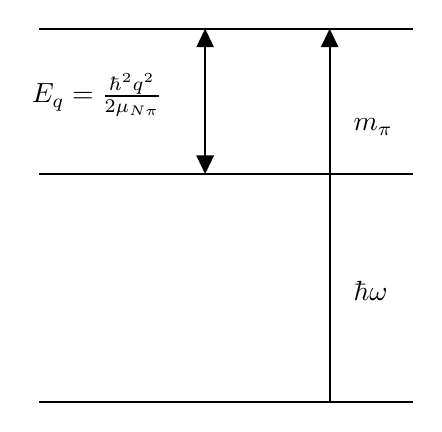
\begin{tikzpicture}[x=0.75pt,y=0.75pt,yscale=-1,xscale=1]
	%uncomment if require: \path (0,300); %set diagram left start at 0, and has height of 300
	
	%Straight Lines [id:da9050164165880492] 
	\draw    (210,200) -- (390,200) ;
	%Straight Lines [id:da595724624922532] 
	\draw    (210,90) -- (390,90) ;
	%Straight Lines [id:da8326738532712242] 
	\draw    (210,20) -- (390,20) ;
	%Straight Lines [id:da4515077860512252] 
	\draw    (350,200) -- (350,23) ;
	\draw [shift={(350,20)}, rotate = 90] [fill={rgb, 255:red, 0; green, 0; blue, 0 }  ][line width=0.08]  [draw opacity=0] (8.93,-4.29) -- (0,0) -- (8.93,4.29) -- cycle    ;
	%Straight Lines [id:da5226155750538098] 
	\draw    (290,87) -- (290,23) ;
	\draw [shift={(290,20)}, rotate = 90] [fill={rgb, 255:red, 0; green, 0; blue, 0 }  ][line width=0.08]  [draw opacity=0] (8.93,-4.29) -- (0,0) -- (8.93,4.29) -- cycle    ;
	\draw [shift={(290,90)}, rotate = 270] [fill={rgb, 255:red, 0; green, 0; blue, 0 }  ][line width=0.08]  [draw opacity=0] (8.93,-4.29) -- (0,0) -- (8.93,4.29) -- cycle    ;
	
	% Text Node
	\draw (360,140) node [anchor=north west][inner sep=0.75pt]    {$\hbar \omega $};
	% Text Node
	\draw (360,62) node [anchor=north west][inner sep=0.75pt]    {$m_{\pi }$};
	% Text Node
	\draw (205,40) node [anchor=north west][inner sep=0.75pt]    {$E_{q} =\frac{\hbar ^{2} q^{2}}{2\mu _{N\pi }}$};
	
	
\end{tikzpicture}
	\caption{Energy diagram of the system. Here $\mu_{N\pi}$ is the reduced mass of the pion-nucleon system.}
	\label{fig:qenergy}
\end{marginfigure}
The final state consists of the unbound system represented by $\psi$. We know the final state consists of a plane wave with wave number $\vec{q}$ propagating along the $z$-axis. The wave number \vec{q} is written in terms of the pion-nucleon momentum, and the magnitude of this is given by
\begin{equation}\label{qenergi}
	\frac{\hbar^2 q^2}{2\mu_{N\pi}}=\hbar \omega-m_\pi c^2,
\end{equation}
which is also illustrated in figure \ref{fig:qenergy}. Equation \eqref{qenergi} also represents the fact that the energy of the photon must be larger than the mass of the pion to disintegrate the pion-nucleon system. Using the wave number $q$, the plane wave can be written as 
\begin{equation} \label{key}
	\text{e}^{iqz} = \text{e}^{i \vec{q}\cdot \vec{r}},
\end{equation}
where $\theta$ is the angle between $\vec{q}$ and $\vec{r}$. Using orthogonality and the addition theorem for the spherical harmonics, we can decompose the plane wave into a Bessel function and spherical harmonics\footnote{See equation \eqref{sphericalbesseldecomp}}. This yields
\begin{align}\label{planewaveexpansion}
	\frac{1}{\sqrt{V}} \text{e}^{-i\vec{q}\cdot\vec{r}} &= \frac{1}{\sqrt{V}} \sum_{\ell,m} 4\pi i^\ell Y_\ell^{*m}(\vec{q})Y_\ell^m(\vec{r})j_\ell(qr) \\
	&= \frac{1}{\sqrt{V}} \sum_\ell 4\pi i^\ell j_\ell(qr) \bigg( \frac{2\ell+1}{4\pi}\bigg)P_\ell(\cos\theta),
\end{align}
where $P_\ell$ is the Legendre polynomial of degree $\ell$. Since we are considering the energies close to the threshold, we expect mainly the $S$-wave to contribute and ignore higher orders\footnote{Threshold behaviour when $\lambda\simeq1/q\gg R$ where $R$ is the range. Higher orders of $\ell$ are generally not important \cite{Sakurai}.}. We should emphasise that this is an approximation, and a priori, we do not know to what degree this holds. In terms of the expansion \eqref{planewaveexpansion}, this greatly simplified the expression
\begin{equation} \label{expansion}
	\frac{1}{\sqrt{V}}\text{e}^{i\vec{q}\cdot \vec{r}} \stackrel{\ell=0}{=} \frac{1}{\sqrt{V}}j_0(qr).
\end{equation}
As equation \eqref{expansion} shows, we are left with a spherical Bessel function in the final state where the volume is kept to stress that the total cross section must be independent of the volume. To compute the matrix element, we return to equation \eqref{quantised} and consider the electric field given by
\begin{equation}\label{EF}
	\vec{\mathcal{E}} = -\frac{1}{c} \frac{\partial \vec{A}}{\partial t}.
\end{equation}
The interaction operator in the dipole approximation is given by
\begin{equation}\label{Dip}
	H_\text{dipole} = -\vec{\mathcal{E}}(\vec{r}=0)\cdot \vec{d},
\end{equation}
where $\vec{d}$ is the dipole moment of the pion-nucleon system given by 
\begin{equation}\label{dipolemoment}
	\vec{d}=e\frac{\mu_{N\pi}}{m_\pi}\vec{r}.
\end{equation}
\begin{marginfigure}
	\centering
	

\tikzset{every picture/.style={line width=0.75pt}} %set default line width to 0.75pt        

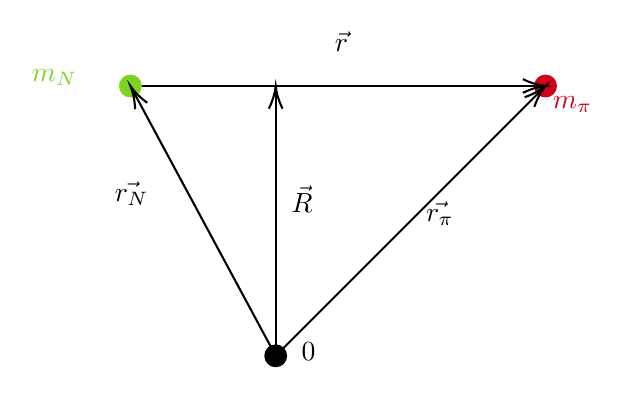
\begin{tikzpicture}[x=0.75pt,y=0.75pt,yscale=-1,xscale=1]
	%uncomment if require: \path (0,300); %set diagram left start at 0, and has height of 300
	
	%Flowchart: Connector [id:dp9827455772611288] 
	\draw  [color={rgb, 255:red, 208; green, 2; blue, 27 }  ,draw opacity=1 ][fill={rgb, 255:red, 208; green, 2; blue, 27 }  ,fill opacity=1 ] (315,90) .. controls (315,87.24) and (317.24,85) .. (320,85) .. controls (322.76,85) and (325,87.24) .. (325,90) .. controls (325,92.76) and (322.76,95) .. (320,95) .. controls (317.24,95) and (315,92.76) .. (315,90) -- cycle ;
	%Straight Lines [id:da5093684133345362] 
	\draw    (125,90) -- (318,90) ;
	\draw [shift={(320,90)}, rotate = 180] [color={rgb, 255:red, 0; green, 0; blue, 0 }  ][line width=0.75]    (10.93,-3.29) .. controls (6.95,-1.4) and (3.31,-0.3) .. (0,0) .. controls (3.31,0.3) and (6.95,1.4) .. (10.93,3.29)   ;
	%Straight Lines [id:da04984112064582158] 
	\draw    (190,220) -- (190,92) ;
	\draw [shift={(190,90)}, rotate = 90] [color={rgb, 255:red, 0; green, 0; blue, 0 }  ][line width=0.75]    (10.93,-3.29) .. controls (6.95,-1.4) and (3.31,-0.3) .. (0,0) .. controls (3.31,0.3) and (6.95,1.4) .. (10.93,3.29)   ;
	%Straight Lines [id:da13661676787341415] 
	\draw    (190,220) -- (318.59,91.41) ;
	\draw [shift={(320,90)}, rotate = 135] [color={rgb, 255:red, 0; green, 0; blue, 0 }  ][line width=0.75]    (10.93,-3.29) .. controls (6.95,-1.4) and (3.31,-0.3) .. (0,0) .. controls (3.31,0.3) and (6.95,1.4) .. (10.93,3.29)   ;
	%Flowchart: Connector [id:dp37210275318157304] 
	\draw  [color={rgb, 255:red, 126; green, 211; blue, 33 }  ,draw opacity=1 ][fill={rgb, 255:red, 126; green, 211; blue, 33 }  ,fill opacity=1 ] (115,90) .. controls (115,87.24) and (117.24,85) .. (120,85) .. controls (122.76,85) and (125,87.24) .. (125,90) .. controls (125,92.76) and (122.76,95) .. (120,95) .. controls (117.24,95) and (115,92.76) .. (115,90) -- cycle ;
	%Straight Lines [id:da8769015497622031] 
	\draw    (190,220) -- (120.95,91.76) ;
	\draw [shift={(120,90)}, rotate = 61.7] [color={rgb, 255:red, 0; green, 0; blue, 0 }  ][line width=0.75]    (10.93,-3.29) .. controls (6.95,-1.4) and (3.31,-0.3) .. (0,0) .. controls (3.31,0.3) and (6.95,1.4) .. (10.93,3.29)   ;
	%Flowchart: Connector [id:dp5562170943538245] 
	\draw  [color={rgb, 255:red, 0; green, 0; blue, 0 }  ,draw opacity=1 ][fill={rgb, 255:red, 0; green, 0; blue, 0 }  ,fill opacity=1 ] (185,220) .. controls (185,217.24) and (187.24,215) .. (190,215) .. controls (192.76,215) and (195,217.24) .. (195,220) .. controls (195,222.76) and (192.76,225) .. (190,225) .. controls (187.24,225) and (185,222.76) .. (185,220) -- cycle ;
	
	% Text Node
	\draw (71,80.4) node [anchor=north west][inner sep=0.75pt]  [color={rgb, 255:red, 126; green, 211; blue, 33 }  ,opacity=1 ]  {$m_{N}$};
	% Text Node
	\draw (322,93.4) node [anchor=north west][inner sep=0.75pt]  [color={rgb, 255:red, 208; green, 2; blue, 27 }  ,opacity=1 ]  {$m_{\pi }$};
	% Text Node
	\draw (196,136.4) node [anchor=north west][inner sep=0.75pt]    {$\vec{R}$};
	% Text Node
	\draw (261,144.4) node [anchor=north west][inner sep=0.75pt]    {$\vec{r_{\pi }}$};
	% Text Node
	\draw (111,134.4) node [anchor=north west][inner sep=0.75pt]    {$\vec{r_{N}}$};
	% Text Node
	\draw (217,62.4) node [anchor=north west][inner sep=0.75pt]    {$\vec{r}$};
	% Text Node
	\draw (201,212.4) node [anchor=north west][inner sep=0.75pt]    {$0$};
	
	
\end{tikzpicture}
	\caption{Relative coordinates of the pion-nucleon system.}
	\label{JacobiIllustration1}
\end{marginfigure}
The general setup for the system is shown in figure \ref{JacobiIllustration1}, where the nucleon, in this case, is a proton. Considering a general pion photoproduction process on the form
\begin{equation}\label{General}
	N+\gamma \rightarrow N+\pi
\end{equation}
allows us to compute the electromagnetic part of the matrix element. The initial state consists of the dressed nucleon, and a photon $a_{\vec{k},\lambda}^\dagger \ket{0}$, where $\ket{0}$ is the electromagnetic vacuum state, $\vec{k}$ is the wave number and $\lambda$ the polarisation index. The final state consists of a nucleon, a pion and the electromagnetic vacuum. This means the transition in the dipole approximation is given by 
\begin{equation}\label{Dip2}
	\mel{0}{\vec{\mathcal{E}}a_{\vec{k},\lambda}^\dagger}{0} = \sqrt{\frac{2\pi\hbar}{\omega_k V}}i\omega_k \vec{e}_{\vec{k},\lambda}\text{e}^{-i\omega_k t},
\end{equation}
which combined with Fermi's golden rule
\begin{equation}\label{FermiGoldenRule}
	\text{d}\omega = \frac{2\pi}{\hbar}\abs{\mathcal{M}}^2 \rho,
\end{equation}
describes the probability per unit of time of making a transition. Equation \eqref{Dip2} is the most general expression we can make, and in this section, consider the $S$-wave channel for the process \eqref{photonew2}. Computations for \eqref{photonew1}, \eqref{photonew3} and \eqref{photonew4} are very similar. Computing the matrix element
\begin{equation}\label{Hdip}
	\mathcal{M}=\mel*{\frac{j_0(qr)}{\sqrt{V}}n\pi^+(\uparrow\downarrow)}{H_\text{dipole}}{\psi_{N\pi}\mathcal{N}}
\end{equation}
Plugging in equation \eqref{Hdip} and \eqref{finalphi}
\begin{align}
	\mathcal{M} =-i\omega_k\sqrt{\frac{2\pi\hbar}{V\omega_{\vec{k}}}}\vec{e}_{\vec{k},\lambda}\mel*{\frac{1}{\sqrt{V}} j_0(qr)n\pi^+ (\uparrow \downarrow)}{\vec{d}}{(\vec{\tau}\cdot \vec{\pi})(\vec{\sigma}\cdot \vec{r})p\uparrow \phi(r)\mathcal{N}}
\end{align}
where the two arrows represent the two spin states of the neutron and the proton. The different spin states of the neutron in the final state yield two contributions to the total matrix element given by
\begin{align}
	\mathcal{M}^{\uparrow} %&=\frac{-i\mathcal{N}\sqrt{2}\omega_k\vec{e}_{\vec{k},\lambda}}{V}\sqrt{\frac{2\pi\hbar}{V\omega_{\vec{k}}}}\mel*{j_0(qr)}{d_0 r_0}{\phi(r)}  \\
	&= \frac{-i\mathcal{N}\sqrt{2}\omega_k\vec{e}_{\vec{k},\lambda}}{V}\sqrt{\frac{2\pi\hbar}{V\omega_{\vec{k}}}}\sqrt{\frac{4\pi}{3}}\mel*{j_0(qr)}{d_0 r Y_1^0}{\phi(r)} \\
	\mathcal{M}^{\downarrow}  % & =\frac{-i\mathcal{N}2\omega_k\vec{e}_{\vec{k},\lambda}}{V}\sqrt{\frac{2\pi\hbar}{V\omega_{\vec{k}}}} \mel{j_0(qr)}{d r_{+}}{\phi(r)}\\
	&=\frac{-i\mathcal{N}2\omega_k\vec{e}_{\vec{k},\lambda}}{V}\sqrt{\frac{2\pi\hbar}{V\omega_{\vec{k}}}}\sqrt{\frac{4\pi}{3}}\mel*{j_0(qr)}{d_0 r Y_1^1}{\phi(r)}, 
\end{align}
where the spin-down state picks up a factor $\sqrt{2}$ from equation \eqref{spinmatrix}. Now we compute the remaining matrix elements,
\begin{align}
	\mel{j_0(qr)}{d_0 r_0}{\phi(r)} &= \frac{\mu_{N\pi}}{m_\pi}e \mel{j_0(qr)}{r_0r_0}{\phi(r)} \\
	&= \frac{\mu_{N\pi}}{m_\pi}e\frac{4\pi}{3} \mel{j_0}{r^2}{\phi(r)} \\
	%&= \frac{\mu e }{m_\pi} \int_0^\pi \int_0^{2\pi} \int_0^\infty \text{d}r \text{d}\phi \text{d}\theta \, j_0(qr)r^4\cos^2\theta \sin\theta \phi(r) \\
	&= \frac{4\pi \mu_{N\pi} e}{3m_\pi} \underbrace{\int_0^\infty \text{d}r \, j_0(qr)r^4\phi(r)}_{\mathcal{Q}(r)}, \label{Matrix1}
\end{align}
where the dipole operator \eqref{dipolemoment} has been inserted and the angular integrals evaluated. We have also introduced an integral, which contains the wave function $\phi(r)$. Similarly, for the next matrix element,
\begin{align}
	\mel{j_0(qr)}{d_{-}r_{+}}{\phi(r)} &= \frac{\mu}{m_\pi}e \mel{j_0(qr)}{r_{-}r_{+}}{\phi(r)} \\
	&= \frac{4\pi \mu e}{3 m_\pi} \mel{j_0(qr)}{r^2 Y_1^{-1}Y_1^1}{\phi(r)} \\
	&= \frac{4\pi \mu e}{3 m_\pi} \mathcal{Q}(r). \label{Matrix2}
\end{align}
It turns out that these two matrix elements are equal. Taking the norm-square of \eqref{Matrix1}
\begin{equation}
	\abs{\mathcal{M}^\uparrow}^2 = \bigg( \frac{4\pi \mu e}{3m_\pi}\bigg)^2 \frac{2 \mathcal{N}^2\omega_k (2\pi \hbar)}{V^2}(\vec{e}_{\vec{k},\lambda})^0(\vec{e}_{\vec{k},\lambda}^*)^0 \mathcal{Q}(r)^2 
\end{equation}
Similarly, for the equation \eqref{Matrix2}
\begin{equation}
	\abs{\mathcal{M}^\downarrow}^2 = \bigg( \frac{4\pi \mu e}{3 m_\pi}\bigg)^2 \frac{4\mathcal{N}\omega_{\vec{k}}(2\pi\hbar)}{V^2}(\vec{e}_{\vec{k},\lambda})^+(\vec{e}_{\vec{k},\lambda}^*)^+ \mathcal{Q}(r)^2.
\end{equation}
Computing the total matrix element using a polarization theorem\footnote{$(\vec{e}_{\vec{k},\lambda}^*\cdot \vec{e}_{\vec{k},\lambda})=\delta_{\lambda,\lambda'}$ and $\vec{e}_{\vec{k},\mp}=\pm\frac{1}{\sqrt{2}}(\vec{e}_{\vec{k},1}\pm i\vec{e}_{\vec{k},2})$. This leads to $(\vec{e}^{0*}_{\vec{k},\lambda}\cdot\vec{e}^{0}_{\vec{k},\lambda'})+(\vec{e}^{0+}_{\vec{k},\lambda}\cdot\vec{e}^{+}_{\vec{k},\lambda'})=\delta_{\lambda,\lambda'}+\frac{1}{2}\delta_{\lambda,\lambda'}$}
\begin{align}
	\abs{\mathcal{M}}^2 &= \abs{\mathcal{M}^\uparrow}^2 + \abs{\mathcal{M}^\downarrow}^2 \\
	&= \frac{2\pi \hbar \omega_k \mathcal{N}^2 e^2}{V^2} \bigg( \frac{4\pi\mu}{3m_\pi}\bigg)^2 \mathcal{Q}(r)^2,
\end{align}
which is the final expression for the matrix element. According to Fermi's golden rule \eqref{FermiGoldenRule} and the non-relativistic density of states \eqref{nonreladensity}, we get the transition probability.
To go from the transition probability to the differential cross-section, we need to consider the flux density of the photons. This means a factor of $V/c$. This leads to the final expressions for the differential cross-section.
\begin{equation}\label{diffcrosssection}
	\frac{\text{d}\sigma^+}{\text{d}\Omega_q}=\frac{16 \pi}{9} \mathcal{N}^2 \alpha\frac{kq\mu^3_{N\pi}}{m_\pi^2 \hbar c}\mathcal{Q}(r)^2,
\end{equation}
where the $+$ is used to indicate that this is the expression for positively charged pions in the final state. Since there is no explicit angular dependency, the total cross-section is given by
\begin{align} 
	\sigma_\text{dipole}^+ & = \oint_{4\pi} \frac{\text{d}\sigma}{\text{d}\Omega_q} \text{d}\Omega_q \\
	%&= 4\pi \frac{16 \pi}{9} \mathcal{N}^2 \alpha\frac{kq\mu^3_{N\pi}}{m_\pi^2 \hbar c}\mathcal{Q}(r)^2 \\
	&= \frac{64\pi^2}{9}\mathcal{N}^2 \alpha \frac{kq\mu^3_{N\pi}}{m_\pi^2 \hbar c} \left( \int_0^\infty \text{d}r \, j_0(qr)r^4 \phi(r)\right)^2 \label{dipoletotalcross}.
\end{align}
This is the final expression for the total cross-section of the photoproduction of charged pions using the dipole approximation. We now perform a fit to experimental data for the parameters $S$ and $b$ that enter in the wave function $\phi(r)$. Here two considerations are needed. Both the dipole approximation and the one-pion approximation limit the validity of the cross-section to near the threshold. Quantitatively the dipole approximation holds when 
\begin{equation}\label{dipoleapprox}
	\lambda \simeq 1/q \gg R,
\end{equation}
where $R$ is the range of the system. In nuclei, the condition \eqref{dipoleapprox} is equivalent to 
\begin{equation}\label{dipolenuc}
	\hbar \omega \ll 165 A^{1/3},
\end{equation}
where $A$ is the nucleon number. This limits our dipole approximation's area of validity to approximately $15$ MeV from the threshold. Equation \eqref{dipoletotalcross} is fitted to experimental data for the parameters $S$ and $b$ using \cite{Scipy,LMfit}. The results are shown in figure \ref{fig:dipolefit}. Data is from \cite{PionOffNeutron}.
\begin{figure}[H]
	\begin{sidecaption}{The total cross-section of the photoproduction process $\gamma p \rightarrow \pi^+ n$ fitted to experimental data. The fit parameters are shown in the figure. The blue data points are included in the fit, and the black data points are excluded since these violate both the dipole and the one-pion approximation. Data is from \cite{PionOffNeutron}}[fig:dipolefit]
		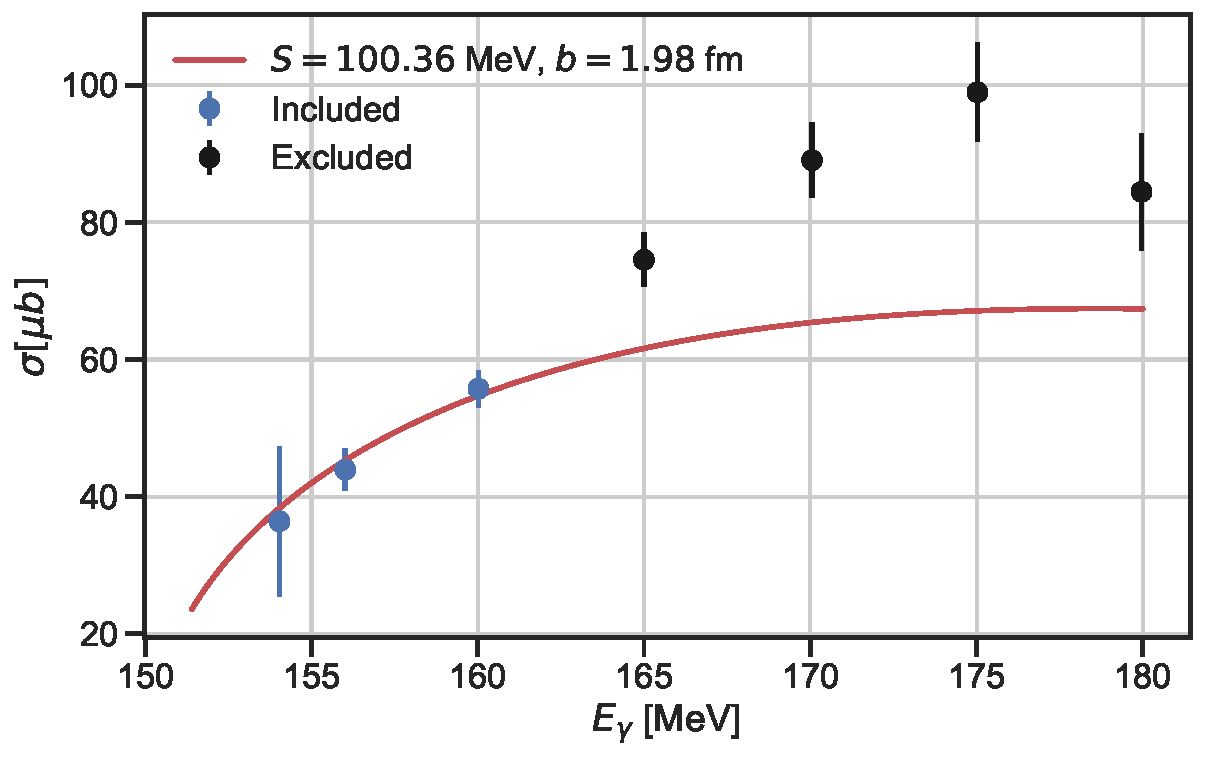
\includegraphics[width=\linewidth]{Figures/dipole_approximation.pdf}
	\end{sidecaption}
\end{figure}
Note here that we have used two approximations that limit \eqref{dipoletotalcross} to energies very close to the threshold. We need a more general expression for the cross-section and more data points to test the model's validity further. This means we have to consider the exact matrix element for the transition and consider the photoproduction of neutral pions off protons since this is the most experimentally investigated photoproduction process. 
\section{Exact Matrix Element}\label{sec:exact}
In section \ref{sec:dipoleapprox}, we investigated how to use the model described in section \ref{sec:model} to get an expression for the cross-section, which was compared to experimental data. More specifically, we used the dipole approximation, which introduces a trade-off between the difficulty of the computations and the regime in which our solution is valid. We expect the dipole approximation to hold for energies just above the threshold. To both validate and generalise this result, we now take a different approach and compute the exact cross-section and also consider recoil effects and apply this approach to the four photoproduction processes using the density of states in the non-relativistic and relativistic limits. Strictly speaking, recoil effects should also be considered in section \ref{sec:dipoleapprox} since the mass ratio between the nucleon and the pion cannot be assumed to yield a stationary nucleon after the pion photoproduction process.  
\begin{marginfigure}
	\centering
	

\tikzset{every picture/.style={line width=0.75pt}} %set default line width to 0.75pt        

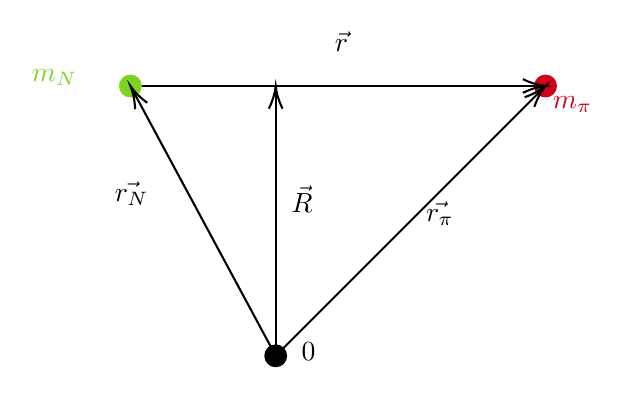
\begin{tikzpicture}[x=0.75pt,y=0.75pt,yscale=-1,xscale=1]
	%uncomment if require: \path (0,300); %set diagram left start at 0, and has height of 300
	
	%Flowchart: Connector [id:dp9827455772611288] 
	\draw  [color={rgb, 255:red, 208; green, 2; blue, 27 }  ,draw opacity=1 ][fill={rgb, 255:red, 208; green, 2; blue, 27 }  ,fill opacity=1 ] (315,90) .. controls (315,87.24) and (317.24,85) .. (320,85) .. controls (322.76,85) and (325,87.24) .. (325,90) .. controls (325,92.76) and (322.76,95) .. (320,95) .. controls (317.24,95) and (315,92.76) .. (315,90) -- cycle ;
	%Straight Lines [id:da5093684133345362] 
	\draw    (125,90) -- (318,90) ;
	\draw [shift={(320,90)}, rotate = 180] [color={rgb, 255:red, 0; green, 0; blue, 0 }  ][line width=0.75]    (10.93,-3.29) .. controls (6.95,-1.4) and (3.31,-0.3) .. (0,0) .. controls (3.31,0.3) and (6.95,1.4) .. (10.93,3.29)   ;
	%Straight Lines [id:da04984112064582158] 
	\draw    (190,220) -- (190,92) ;
	\draw [shift={(190,90)}, rotate = 90] [color={rgb, 255:red, 0; green, 0; blue, 0 }  ][line width=0.75]    (10.93,-3.29) .. controls (6.95,-1.4) and (3.31,-0.3) .. (0,0) .. controls (3.31,0.3) and (6.95,1.4) .. (10.93,3.29)   ;
	%Straight Lines [id:da13661676787341415] 
	\draw    (190,220) -- (318.59,91.41) ;
	\draw [shift={(320,90)}, rotate = 135] [color={rgb, 255:red, 0; green, 0; blue, 0 }  ][line width=0.75]    (10.93,-3.29) .. controls (6.95,-1.4) and (3.31,-0.3) .. (0,0) .. controls (3.31,0.3) and (6.95,1.4) .. (10.93,3.29)   ;
	%Flowchart: Connector [id:dp37210275318157304] 
	\draw  [color={rgb, 255:red, 126; green, 211; blue, 33 }  ,draw opacity=1 ][fill={rgb, 255:red, 126; green, 211; blue, 33 }  ,fill opacity=1 ] (115,90) .. controls (115,87.24) and (117.24,85) .. (120,85) .. controls (122.76,85) and (125,87.24) .. (125,90) .. controls (125,92.76) and (122.76,95) .. (120,95) .. controls (117.24,95) and (115,92.76) .. (115,90) -- cycle ;
	%Straight Lines [id:da8769015497622031] 
	\draw    (190,220) -- (120.95,91.76) ;
	\draw [shift={(120,90)}, rotate = 61.7] [color={rgb, 255:red, 0; green, 0; blue, 0 }  ][line width=0.75]    (10.93,-3.29) .. controls (6.95,-1.4) and (3.31,-0.3) .. (0,0) .. controls (3.31,0.3) and (6.95,1.4) .. (10.93,3.29)   ;
	%Flowchart: Connector [id:dp5562170943538245] 
	\draw  [color={rgb, 255:red, 0; green, 0; blue, 0 }  ,draw opacity=1 ][fill={rgb, 255:red, 0; green, 0; blue, 0 }  ,fill opacity=1 ] (185,220) .. controls (185,217.24) and (187.24,215) .. (190,215) .. controls (192.76,215) and (195,217.24) .. (195,220) .. controls (195,222.76) and (192.76,225) .. (190,225) .. controls (187.24,225) and (185,222.76) .. (185,220) -- cycle ;
	
	% Text Node
	\draw (71,80.4) node [anchor=north west][inner sep=0.75pt]  [color={rgb, 255:red, 126; green, 211; blue, 33 }  ,opacity=1 ]  {$m_{N}$};
	% Text Node
	\draw (322,93.4) node [anchor=north west][inner sep=0.75pt]  [color={rgb, 255:red, 208; green, 2; blue, 27 }  ,opacity=1 ]  {$m_{\pi }$};
	% Text Node
	\draw (196,136.4) node [anchor=north west][inner sep=0.75pt]    {$\vec{R}$};
	% Text Node
	\draw (261,144.4) node [anchor=north west][inner sep=0.75pt]    {$\vec{r_{\pi }}$};
	% Text Node
	\draw (111,134.4) node [anchor=north west][inner sep=0.75pt]    {$\vec{r_{N}}$};
	% Text Node
	\draw (217,62.4) node [anchor=north west][inner sep=0.75pt]    {$\vec{r}$};
	% Text Node
	\draw (201,212.4) node [anchor=north west][inner sep=0.75pt]    {$0$};
	
	
\end{tikzpicture}
	\caption{Sketch of the system. Here $\vec{r}_N$ is the coordinate of the proton and $\vec{r}_\pi$ is the coordinate of the pion. The relative coordinate is given by $\vec{r}=\vec{r}_\pi-\vec{r}_N$ and the coordinate of the center-of-mass is $\vec{R}=(m_N \vec{r}_N+m_\pi\vec{r}_\pi)/(m_N+m_\pi)$. The total mass is denoted $M_{N\pi}=m_N+m_\pi$.}
	\label{JacobiIllustration}
\end{marginfigure}
To compute the exact matrix elements, we consider a non-relativistic system of particles interacting with the electromagnetic field as described in section \ref{RadMatter}. We have to remember that equation \eqref{RadiationHamil} describes how a particle with charge interacts with the electromagnetic field. If we consider a process where the initial state is a dressed neutron, the pion must be responsible for the interaction with the electromagnetic field. We will consider the four pion photoproduction processes separately even though the computations are very similar. In general, we will consider a system illustrated in figure \ref{JacobiIllustration}, which shows the pion-nucleon system, and in terms of the Jacobi coordinates, we get the following expressions for the coordinates of the particles
\begin{align} \label{Coordinates}
	\vec{r}_N = \vec{R}-\frac{m_\pi}{M_{N\pi}}\vec{r} \\
	\vec{r}_\pi = \vec{R}+\frac{m_N}{M_{N\pi}}\vec{r},
\end{align}
where $\vec{R}$ is the coordinate of the center of mass of the pion-nucleon system given by
\begin{equation} \label{Rvec}
	\vec{R}=\frac{m_N \vec{r}_N+m_\pi \vec{r}_\pi}{M_{N\pi}}, \quad M_{N\pi} = m_N+m_\pi.
\end{equation}
The relative coordinate is given by
\begin{equation} \label{rvec}
	\vec{r} = \vec{r}_\pi-\vec{r}_N.
\end{equation}
The general approach is the same as in section \ref{sec:DressingofProton}, where we want to use Fermi's golden rule to compute the total cross-section. In this section, we also consider the impact of changing the density of states to the relativistic case. Furthermore, we estimate the relative weight of the pion component in the wave function of the dressed nucleon. We do this by introducing the following
\begin{equation} \label{relativeweight}
	C(\psi_{N\pi}) = \int_V \text{d}^3 R \int_V \text{d}^3 r \, \abs{\psi_{N\pi}}^2,
\end{equation}
where per construction of the model, this is dimensionless. We also introduce a parameter to estimate the virtual pions' contribution to the mass of the dressed nucleon. This will be denoted $\Pi$ and corresponds to the energy found by solving \eqref{system}.

\subsection{Neutral Pion Photoproduction off Protons}\label{sec:NeutralOffProton}
We are considering the process
\begin{equation} \label{prod1}
	p\gamma \rightarrow \pi^0 p,
\end{equation}
where the proton interacts with the electromagnetic field. The Feynman diagram is shown in figure \ref{Feynman1}. From equation \eqref{RadiationHamil} we get
\begin{equation} \label{1trans}
	H^{(1)} = -\frac{e}{m_pc} \vec{A}(\vec{r}_p,t)\cdot \vec{p}_p,
\end{equation}
\begin{marginfigure}
	\centering
	

\tikzset{every picture/.style={line width=0.75pt}} %set default line width to 0.75pt        

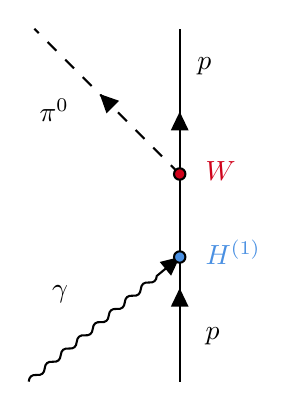
\begin{tikzpicture}[x=0.75pt,y=0.75pt,yscale=-1,xscale=1]
	%uncomment if require: \path (0,300); %set diagram left start at 0, and has height of 300
	
	%Straight Lines [id:da33488681649693186] 
	\draw    (270,210) -- (270,130) ;
	\draw [shift={(270,165)}, rotate = 90] [fill={rgb, 255:red, 0; green, 0; blue, 0 }  ][line width=0.08]  [draw opacity=0] (8.93,-4.29) -- (0,0) -- (8.93,4.29) -- cycle    ;
	%Straight Lines [id:da46389908648611555] 
	\draw    (197.25,210) .. controls (197.48,207.65) and (198.76,206.59) .. (201.11,206.82) .. controls (203.46,207.05) and (204.74,205.99) .. (204.96,203.64) .. controls (205.19,201.29) and (206.47,200.23) .. (208.82,200.46) .. controls (211.17,200.68) and (212.45,199.62) .. (212.68,197.27) .. controls (212.91,194.92) and (214.19,193.86) .. (216.54,194.09) .. controls (218.89,194.32) and (220.17,193.26) .. (220.39,190.91) .. controls (220.62,188.56) and (221.9,187.5) .. (224.25,187.73) .. controls (226.6,187.96) and (227.88,186.9) .. (228.11,184.55) .. controls (228.34,182.2) and (229.62,181.14) .. (231.97,181.37) .. controls (234.32,181.6) and (235.6,180.54) .. (235.82,178.19) .. controls (236.05,175.84) and (237.33,174.78) .. (239.68,175.01) .. controls (242.03,175.23) and (243.31,174.17) .. (243.54,171.82) .. controls (243.77,169.47) and (245.05,168.41) .. (247.4,168.64) .. controls (249.75,168.87) and (251.03,167.81) .. (251.25,165.46) .. controls (251.48,163.11) and (252.76,162.05) .. (255.11,162.28) .. controls (257.46,162.51) and (258.74,161.45) .. (258.97,159.1) -- (261.51,157) -- (267.69,151.91) ;
	\draw [shift={(270,150)}, rotate = 140.49] [fill={rgb, 255:red, 0; green, 0; blue, 0 }  ][line width=0.08]  [draw opacity=0] (8.93,-4.29) -- (0,0) -- (8.93,4.29) -- cycle    ;
	%Straight Lines [id:da3810232285211974] 
	\draw  [dash pattern={on 4.5pt off 4.5pt}]  (270,110) -- (200,40) ;
	\draw [shift={(231.46,71.46)}, rotate = 45] [fill={rgb, 255:red, 0; green, 0; blue, 0 }  ][line width=0.08]  [draw opacity=0] (8.93,-4.29) -- (0,0) -- (8.93,4.29) -- cycle    ;
	%Straight Lines [id:da6452866026111611] 
	\draw    (270,130) -- (270,40) ;
	\draw [shift={(270,80)}, rotate = 90] [fill={rgb, 255:red, 0; green, 0; blue, 0 }  ][line width=0.08]  [draw opacity=0] (8.93,-4.29) -- (0,0) -- (8.93,4.29) -- cycle    ;
	%Shape: Circle [id:dp14659197000759305] 
	\draw  [fill={rgb, 255:red, 74; green, 144; blue, 226 }  ,fill opacity=1 ] (267.25,150) .. controls (267.25,148.48) and (268.48,147.25) .. (270,147.25) .. controls (271.52,147.25) and (272.75,148.48) .. (272.75,150) .. controls (272.75,151.52) and (271.52,152.75) .. (270,152.75) .. controls (268.48,152.75) and (267.25,151.52) .. (267.25,150) -- cycle ;
	%Shape: Circle [id:dp1667146356512621] 
	\draw  [fill={rgb, 255:red, 208; green, 2; blue, 27 }  ,fill opacity=1 ] (267.25,110) .. controls (267.25,108.48) and (268.48,107.25) .. (270,107.25) .. controls (271.52,107.25) and (272.75,108.48) .. (272.75,110) .. controls (272.75,111.52) and (271.52,112.75) .. (270,112.75) .. controls (268.48,112.75) and (267.25,111.52) .. (267.25,110) -- cycle ;
	
	% Text Node
	\draw (281,182.4) node [anchor=north west][inner sep=0.75pt]    {$p$};
	% Text Node
	\draw (277,52.4) node [anchor=north west][inner sep=0.75pt]    {$p$};
	% Text Node
	\draw (201,72.4) node [anchor=north west][inner sep=0.75pt]    {$\pi ^{0}$};
	% Text Node
	\draw (207,162.4) node [anchor=north west][inner sep=0.75pt]    {$\gamma $};
	% Text Node
	\draw (281,140.4) node [anchor=north west][inner sep=0.75pt]  [color={rgb, 255:red, 74; green, 144; blue, 226 }  ,opacity=1 ]  {$H^{( 1)}$};
	% Text Node
	\draw (281,102.4) node [anchor=north west][inner sep=0.75pt]  [color={rgb, 255:red, 208; green, 2; blue, 27 }  ,opacity=1 ]  {$W$};
	
	
\end{tikzpicture}
	\caption{Feynman diagram of neutral pion photoproduction off protons. The blue vertex corresponds to equation \eqref{1trans} and the red vertex corresponds to equation \eqref{W}.}
	\label{Feynman1}
\end{marginfigure} 
To calculate the exact matrix el
where $\vec{p}_p$ is the momentum operator of the proton.  Equation \eqref{1trans} can be rewritten in terms of the relative coordinates
\begin{equation} \label{1rela}
	H^{(1)} = -\frac{e}{m_p c}\vec{A}\left( \vec{R}-\frac{m_\pi}{M_{p\pi}}\vec{r,t}\right) \cdot \left( \frac{m_p}{M_{p\pi}}\vec{P}-\vec{p}\right)
\end{equation}
In equation \eqref{prod1}, the initial state consists of a dressed proton and a plane wave photon in the state $a_{\vec{k},\lambda}^\dagger\ket{0}$. The final state consists of a proton and a $\pi^0$ in a relative plane wave motion. The electromagnetic part of the matrix element is
\begin{align} \label{eletrans}
	-\frac{e}{m_p c}\mel{0}{\vec{A}(\vec{r}_p,t)a^\dagger_{\vec{k},\lambda}}{0} &= -\frac{e}{m_p c}\sqrt{\frac{2\pi\hbar}{\omega_k V}}\vec{e}_{\vec{k},\lambda} \text{e}^{i\vec{k}\cdot \vec{r}_p-i\omega_k t} \\
	&=  -\frac{e}{m_p c}\sqrt{\frac{2\pi\hbar}{\omega_k V}}\vec{e}_{\vec{k},\lambda} \text{e}^{i\vec{k}( \vec{R}-\frac{m_\pi}{M_{p\pi}}\vec{r})-i\omega_k t}.
\end{align}
\begin{marginfigure}
	\centering
	

\tikzset{every picture/.style={line width=0.75pt}} %set default line width to 0.75pt        

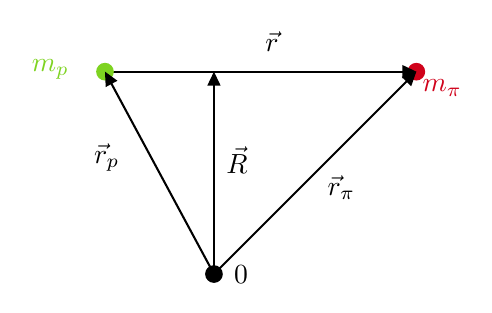
\begin{tikzpicture}[x=0.75pt,y=0.75pt,yscale=-0.75,xscale=0.75]
	%uncomment if require: \path (0,300); %set diagram left start at 0, and has height of 300
	
	%Flowchart: Connector [id:dp9827455772611288] 
	\draw  [color={rgb, 255:red, 208; green, 2; blue, 27 }  ,draw opacity=1 ][fill={rgb, 255:red, 208; green, 2; blue, 27 }  ,fill opacity=1 ] (315,90) .. controls (315,87.24) and (317.24,85) .. (320,85) .. controls (322.76,85) and (325,87.24) .. (325,90) .. controls (325,92.76) and (322.76,95) .. (320,95) .. controls (317.24,95) and (315,92.76) .. (315,90) -- cycle ;
	%Straight Lines [id:da5093684133345362] 
	\draw    (125,90) -- (317,90) ;
	\draw [shift={(320,90)}, rotate = 180] [fill={rgb, 255:red, 0; green, 0; blue, 0 }  ][line width=0.08]  [draw opacity=0] (8.93,-4.29) -- (0,0) -- (8.93,4.29) -- cycle    ;
	%Straight Lines [id:da04984112064582158] 
	\draw    (190,220) -- (190,93) ;
	\draw [shift={(190,90)}, rotate = 90] [fill={rgb, 255:red, 0; green, 0; blue, 0 }  ][line width=0.08]  [draw opacity=0] (8.93,-4.29) -- (0,0) -- (8.93,4.29) -- cycle    ;
	%Straight Lines [id:da13661676787341415] 
	\draw    (190,220) -- (317.88,92.12) ;
	\draw [shift={(320,90)}, rotate = 135] [fill={rgb, 255:red, 0; green, 0; blue, 0 }  ][line width=0.08]  [draw opacity=0] (8.93,-4.29) -- (0,0) -- (8.93,4.29) -- cycle    ;
	%Flowchart: Connector [id:dp37210275318157304] 
	\draw  [color={rgb, 255:red, 126; green, 211; blue, 33 }  ,draw opacity=1 ][fill={rgb, 255:red, 126; green, 211; blue, 33 }  ,fill opacity=1 ] (115,90) .. controls (115,87.24) and (117.24,85) .. (120,85) .. controls (122.76,85) and (125,87.24) .. (125,90) .. controls (125,92.76) and (122.76,95) .. (120,95) .. controls (117.24,95) and (115,92.76) .. (115,90) -- cycle ;
	%Straight Lines [id:da8769015497622031] 
	\draw    (190,220) -- (121.42,92.64) ;
	\draw [shift={(120,90)}, rotate = 61.7] [fill={rgb, 255:red, 0; green, 0; blue, 0 }  ][line width=0.08]  [draw opacity=0] (8.93,-4.29) -- (0,0) -- (8.93,4.29) -- cycle    ;
	%Flowchart: Connector [id:dp5562170943538245] 
	\draw  [color={rgb, 255:red, 0; green, 0; blue, 0 }  ,draw opacity=1 ][fill={rgb, 255:red, 0; green, 0; blue, 0 }  ,fill opacity=1 ] (185,220) .. controls (185,217.24) and (187.24,215) .. (190,215) .. controls (192.76,215) and (195,217.24) .. (195,220) .. controls (195,222.76) and (192.76,225) .. (190,225) .. controls (187.24,225) and (185,222.76) .. (185,220) -- cycle ;
	
	% Text Node
	\draw (71,80.4) node [anchor=north west][inner sep=0.75pt]  [color={rgb, 255:red, 126; green, 211; blue, 33 }  ,opacity=1 ]  {$m_{p}$};
	% Text Node
	\draw (322,93.4) node [anchor=north west][inner sep=0.75pt]  [color={rgb, 255:red, 208; green, 2; blue, 27 }  ,opacity=1 ]  {$m_{\pi }$};
	% Text Node
	\draw (196,136.4) node [anchor=north west][inner sep=0.75pt]    {$\vec{R}$};
	% Text Node
	\draw (261,155) node [anchor=north west][inner sep=0.75pt]    {$\vec{r}_{\pi }$};
	% Text Node
	\draw (111,134.4) node [anchor=north west][inner sep=0.75pt]    {$\vec{r}_{p}$};
	% Text Node
	\draw (221,62.4) node [anchor=north west][inner sep=0.75pt]    {$\vec{r}$};
	% Text Node
	\draw (201,212.4) node [anchor=north west][inner sep=0.75pt]    {$0$};
	
	
\end{tikzpicture}
	\caption{Sketch of the system. Here $\vec{r}_p$ is the coordinate of the proton and $\vec{r}_\pi$ is the coordinate of the pion. The relative coordinate is given by $\vec{r}=\vec{r}_\pi-\vec{r}_p$ and the coordinate of the center-of-mass is $\vec{R}=(m_p \vec{r}_p+m_\pi\vec{r}_\pi)/(m_p+m_\pi)$. The total mass is denoted $M_{p\pi}=m_p+m_\pi$.}
	\label{JacobiIllustrationProton}
\end{marginfigure}
We now return to equation \eqref{1rela} where we set $\vec{P}=0$, which corresponds to moving to the lab frame, and the matrix element needed for Fermi's golden rule is given by
\begin{equation}\label{MatrixSpinupdown} 
	\mathcal{M}^{(\uparrow\downarrow)} = \frac{e}{m_p} \sqrt{\frac{2\pi\hbar}{\omega_{\vec{k}}V}} \mel*{(\uparrow\downarrow)p\pi^0 \frac{\text{e}^{i\vec{q}\cdot \vec{r}}}{\sqrt{V}}\frac{\text{e}^{i\vec{Q}\cdot \vec{r}}}{\sqrt{V}}}{\text{e}^{i\vec{k}(\vec{R}-\frac{m_\pi}{M_{p\pi}}\vec{r})}(\vec{e}_{\vec{k},\lambda}\cdot\vec{p})}{\psi_{N\pi}} ,
\end{equation}
where $\vec{q}$ is the wave number of the relative pion-proton system and $\vec{Q}=\vec{k}$ is the recoil. Looking at the isospin coefficient from equation \eqref{isocoeff}, which is the factor that separates neutral pions from charged pions aside from the mass difference\footnote{$\mel{p\pi^0}{\vec{\tau}\cdot\vec{\pi}}{p}=1$}. Inserting \eqref{pionnuc} and using that volume condition yields the following expression\footnote{$\int \text{d}^3R \, \text{e}^{i\vec{k}\cdot\vec{R}}=V$}
\begin{equation} \label{MatrixSpinupdown2}
	\mathcal{M}^{(\uparrow\downarrow)} = \frac{e}{m_p} \sqrt{\frac{2\pi\hbar}{\omega_{\vec{k}}V}} \mel*{(\uparrow\downarrow)p\pi^0 \frac{\text{e}^{i\vec{q}\cdot \vec{r}}}{\sqrt{V}}}{\text{e}^{-i\frac{m_\pi}{M_{p\pi}}\vec{k}\cdot\vec{r}}(\vec{e}_{\vec{k},\lambda}\cdot\vec{p})}{(\vec{\tau}\cdot\vec{\pi})(\vec{\sigma}\cdot\vec{r})\phi(r) \frac{p\uparrow}{\sqrt{V}}} 
\end{equation}
Defining a new vector, $\vec{s}=\vec{q}+\frac{m_\pi}{M_{p\pi}}\vec{k}$ yields
\begin{equation}\label{doublematrix}
	\mathcal{M}^{(\uparrow\downarrow)} = \frac{-e}{m_\pi} \sqrt{\frac{2\pi\hbar}{\omega_{\vec{k}}}} \frac{1}{V} \mel{(\uparrow \downarrow)}{\mel*{\text{e}^{i\vec{s}\cdot\vec{r}}}{(\vec{e}_{\vec{k},\lambda}\cdot\vec{p})(\vec{\sigma}\cdot\vec{r})}{\phi(r)}}{\uparrow}
\end{equation}
Note the different inner products. We now consider the innermost matrix element in equation \eqref{doublematrix} where the momentum operator is inserted
\begin{align}
	\mel*{\text{e}^{i\vec{s}\cdot\vec{r}}}{(\vec{e}_{\vec{k},\lambda}\frac{\partial}{\partial \vec{r}})\sigmar}{\phi(r)} &=+i(\vec{e}_{\vec{k},\lambda}\cdot \vec{s}) \int \text{d}^3 r \, \text{e}^{i\vec{s}\cdot\vec{r}}\sigmar \phi(r) \\ 
	&= -i(\vec{e}_{\vec{k},\lambda}\cdot \vec{s}) \int \text{d}^3 r \, 3 i j_1(sr) \frac{\vec{s}\cdot \vec{r}}{sr}\sigmar \phi(r)  \label{planebob}\\
	&= (\vec{e}_{\vec{k},\lambda}\cdot \vec{s})\sigmar \underbrace{\frac{4\pi}{s} \int_0^\infty \text{d}r \, r^3 j_1(sr) \phi(r)}_{F(s)} \label{unitbob} \\
	&= (\vec{e}_{\vec{k},\lambda}\cdot \vec{s})\sigmar F(s).
\end{align}
Where we used the spherical Bessel decomposition \eqref{sphericalbesseldecomp} in equation \eqref{planebob}. In equation \eqref{unitbob} we considered the angular averaging of two coordinates variables\footnote{$\int \text{d}\Omega \, n_k n_l =\frac{4\pi}{3}\delta_{kl}$, which means $\int \text{d}\Omega \, r_k r_l =\frac{4\pi r^2}{3}\delta_{kl}$, where $n$ is a unit vector.}.
We now have an expression for the innermost matrix element in equation \eqref{doublematrix}, which depends on the wave function $\phi(r)$. This is where the two parameters $S$ and $b$ enter, and ultimately these are the parameters we want to extract. It should also be noted that $F(s)$ is essentially the Hankel transform of $\phi(r)$\footnote{See appendix \ref{app:Besselfunctions}.}. Returning to the matrix element \eqref{doublematrix}
\begin{align}
	\mathcal{M^{(\uparrow\downarrow)}} &= \frac{ie\hbar}{m_p}\sqrt{\frac{2\pi \hbar}{\omega_k}}\frac{1}{V}\mel*{(\uparrow\downarrow)}{(\vec{e}_{\vec{k},\lambda}\cdot\vec{s})F(s)}{\uparrow} \\
	&=\frac{ie\hbar}{m_p}\sqrt{\frac{2\pi \hbar}{\omega_k}}\frac{1}{V} (\vec{e}_{\vec{k},\lambda}\cdot\vec{s})\mel*{(\uparrow\downarrow)}{\sigmar}{\uparrow}F(s),
\end{align}
which leads to the following expression for the norm square of equation \eqref{doublematrix}. We do this step already to use a completeness relation for the polarisation.
\begin{equation} \label{matrixspinupdownabs}
	\abs{\mathcal{M}^{(\uparrow\downarrow)}}^2 = \frac{2\pi\hbar^3e^2}{m_p^2\omega_k V^2} \abs{\evec\cdot \vec{s}}^2 \abs{\mel*{(\uparrow\downarrow)}{(\vec{\sigma}\cdot \vec{s})}{\uparrow}}^2 F(s)^2,
\end{equation}
and now evaluating
\begin{align} \label{sumoverpol}
	\sum_\lambda \abs{(\evec \cdot \vec{s})}^2 &= \sum_\lambda (\evec^*\cdot \vec{s})(\evec\cdot\vec{s}) \\
	&= s^2 -\frac{(\vec{k}\cdot \vec{s})^2}{k^2} \\
	&= q^2 -\frac{(\vec{k}\cdot \vec{q})^2}{k^2} \\
	&= q^2 \sin^2(\theta_q),\label{finalsum}
\end{align}
where $\theta_q$ is the angle between $\vec{k}$ and $\vec{q}$, and we now have an angular dependency originating from the dot product. This step also assumes the target is unpolarised since we sum over the spin states of the proton. The subscript $q$ is used to emphasise that this is relative to the final state momentum, also mentioned in section \ref{sec:densityofstates}. The final missing term is computed by summing over the final proton spin states using \eqref{spinmatrix}
\begin{equation} \label{spinsum}
	\sum_{(\uparrow\downarrow)} \abs{\mel*{(\uparrow\downarrow)}{(\vec{\sigma}\cdot\vec{s})}{\uparrow}}^2 = s^2
\end{equation}
Using the final two expressions equation \eqref{finalsum} and \eqref{spinsum} with equation \eqref{matrixspinupdownabs} and remembering the factor $1/2$ from the spin states
\begin{equation} \label{absmatrixexact}
	\frac{1}{2}\sum_{\lambda,(\uparrow\downarrow)} \abs{\mathcal{M}_{fi}}^2 = \frac{\pi e^2\hbar^3}{V^2 m_p^2}\frac{1}{\omega_k} q^2\sin^2(\theta) s^2 F(s)^2.
\end{equation}
According to Fermi's golden rule, the transition probability is given by
\begin{align}\label{Fermisgolden}
	\text{d}\omega &= \frac{2\pi}{\hbar}\abs{\mathcal{M}}^2\rho,
\end{align}
where we can use both expressions for the density of states. We can either use the relativistic equation \eqref{derivative} or the non-relativistic equation \eqref{nonreladensity}. We will use the relativistic expression as an example but show both results at the end of the section. This leads to the final transition probability
\begin{equation}
	\text{d}\omega^0 = \frac{e^2c}{8\pi V}\frac{1}{m_p^2 c^4}\frac{\text{d}(\hbar c q)^2}{\text{d}E_q}\frac{q^3}{k} \sin^2(\theta_q) s^2 F(s)^2 \text{d}\Omega_q
\end{equation}
which leads to the following expression for the differential cross section by considering the time it takes the photon to cross the volume, $V$.
\begin{equation}\label{exactdiffcross}
	\frac{\text{d}\sigma^0(E_q,\theta_q)}{\text{d}\Omega_q} = \frac{e^2}{8\pi}\frac{1}{m_p^2c^4}\frac{q^3}{k}\frac{\text{d}(\hbar c q)^2}{\text{d}E_q}\sin^2(\theta_q) s^2 F(s)^2,
\end{equation}
where the superscript is used to indicate the photoproduction of neutral pions. To get the total cross-section, we integrate all angles
\begin{align} \label{exactcross}
	\sigma^0 & = 2\pi \int_0^\pi \text{d}\theta_q \, \sin(\theta_q) \frac{\text{d}\sigma^0}{\text{d}\Omega_q} \\ &= 2\pi \int_0^\pi \text{d}\theta_q \, \frac{e^2}{8\pi}\frac{1}{m_p^2c^4}\frac{q^3}{k}\frac{\text{d}(\hbar c q)^2}{\text{d}E_q}\sin^3(\theta_q) s^2 F(s)^2 \label{finalcrosser}.
\end{align}
Equation \eqref{finalcrosser} might seem easy to compute at first, but we have to remember $F(s)$ also contains an angular dependency originating from the magnitude of $\vec{s}$. Specifically, the term\footnote{Note that equation \eqref{sexpanded} changes according to changes in \eqref{1rela}.}
\begin{equation} \label{sexpanded}
	s = \sqrt{q^2+k^2\bigg(\frac{m_\pi}{M_{p\pi}}\bigg)^2+2qk\frac{m_\pi}{M_{p\pi}}\cos(\theta_q)}
\end{equation}
We now perform a fit of equation \eqref{finalcrosser} to experimental data for the parameters $S$ and $b$ using \cite{Scipy,LMfit}. This is shown in figure \ref{fig:crossfitrel} for the relativistic density of states. Data is from  \cite{Schmidt_2001}.
\begin{figure}[H]
	\begin{sidecaption}{Fitted parameters to experimental data for the process $\gamma p \rightarrow \pi^0 p$ using the relativistic density of states \eqref{derivative}. The fit parameters for $S,b$ are shown inside the figure. Data is from \cite{Schmidt_2001}. The threshold energy for this process is 144.7 MeV.}[fig:crossfitrel]
		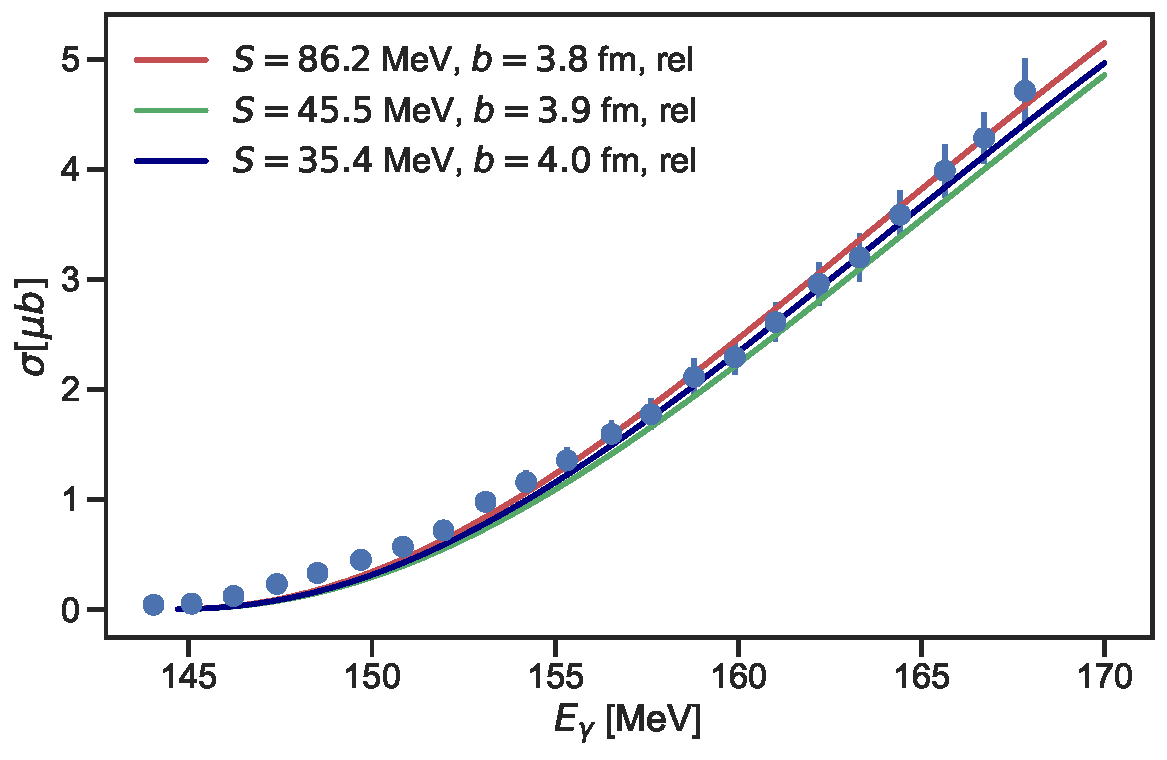
\includegraphics[width=\linewidth]{Figures/crossfit_rel.pdf}
	\end{sidecaption}
\end{figure}
We see that the model with explicit pions can reproduce experimental data for at least three sets of parameters. The same figure can be reproduced for the non-relativistic density of states \eqref{nonreladensity} where the total cross section is given by
\begin{equation} \label{nonrelcrossfit}
	\sigma^0 = 2\pi \int_0^\pi \text{d}\theta_q \, \frac{e^2}{4\pi}\frac{\mu_{p\pi}c^2}{m_p^2 c^4}\frac{q^3}{k}\sin^3(\theta_q)s^2 F(s)^2.
\end{equation} 
This is shown in figure \ref{fig:crossfitnonrel}
\begin{figure}[H]
	\begin{sidecaption}{The same parameters as in figure \ref{fig:crossfitrel} but using the non-relativistic density of states \eqref{nonreladensity}.}[fig:crossfitnonrel]
		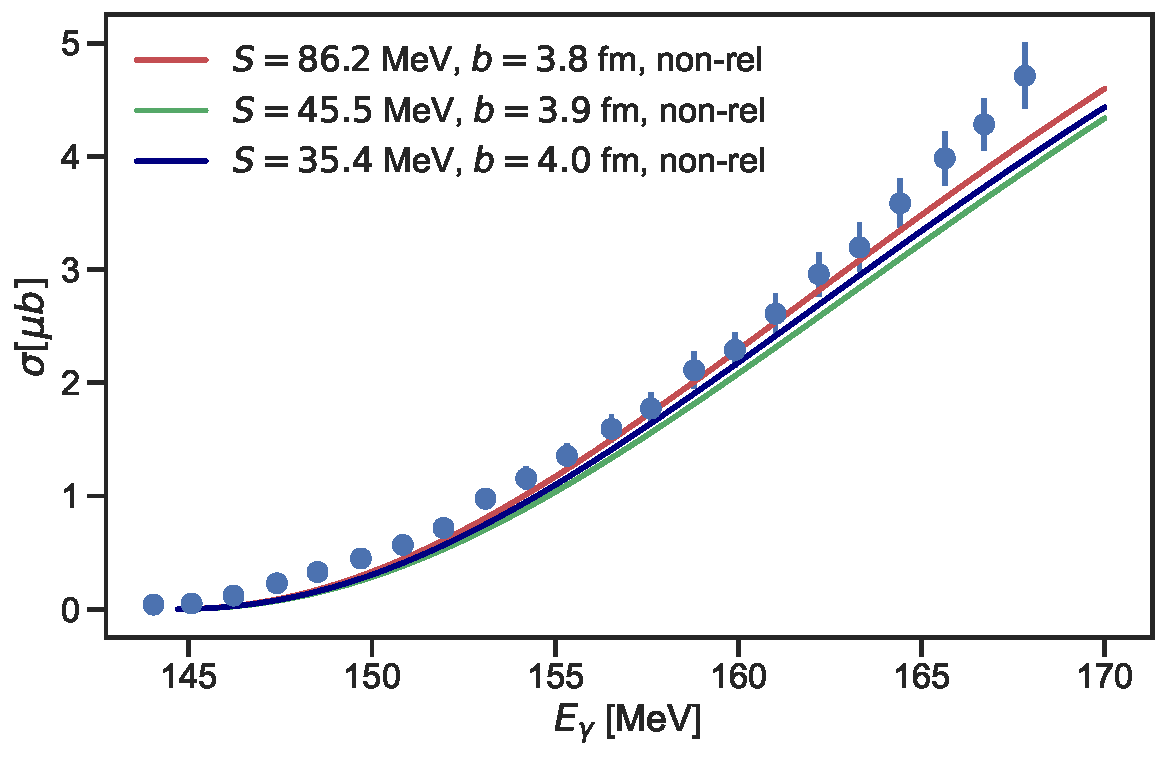
\includegraphics[width=\linewidth]{Figures/crossfit_nonrel.pdf} 
	\end{sidecaption}
\end{figure}
In figure \ref{fig:crossfitnonrel}, the cross-section falls off too quickly compared to figure \ref{fig:crossfitrel}. This indicates relativistic effects become more important as the photon energy increases. 
In equation \eqref{exactdiffcross}, we have an expression for the angular dependency. This means that for some photon energy, we get an angular distribution. Figure \ref{fig:angular151} shows the differential cross section as a function of the angle $\theta_q$ compared to experimental data. Data is from \cite{BeckPion}.  
\begin{figure}[H]
	\begin{sidecaption}{Angular distribution using equation \eqref{exactdiffcross} and experimental data from \cite{BeckPion}.  Note the dependency is not $\sin(\theta_q)^2$ since there is a contribution from $F(s)$ as well.}[fig:angular151]
		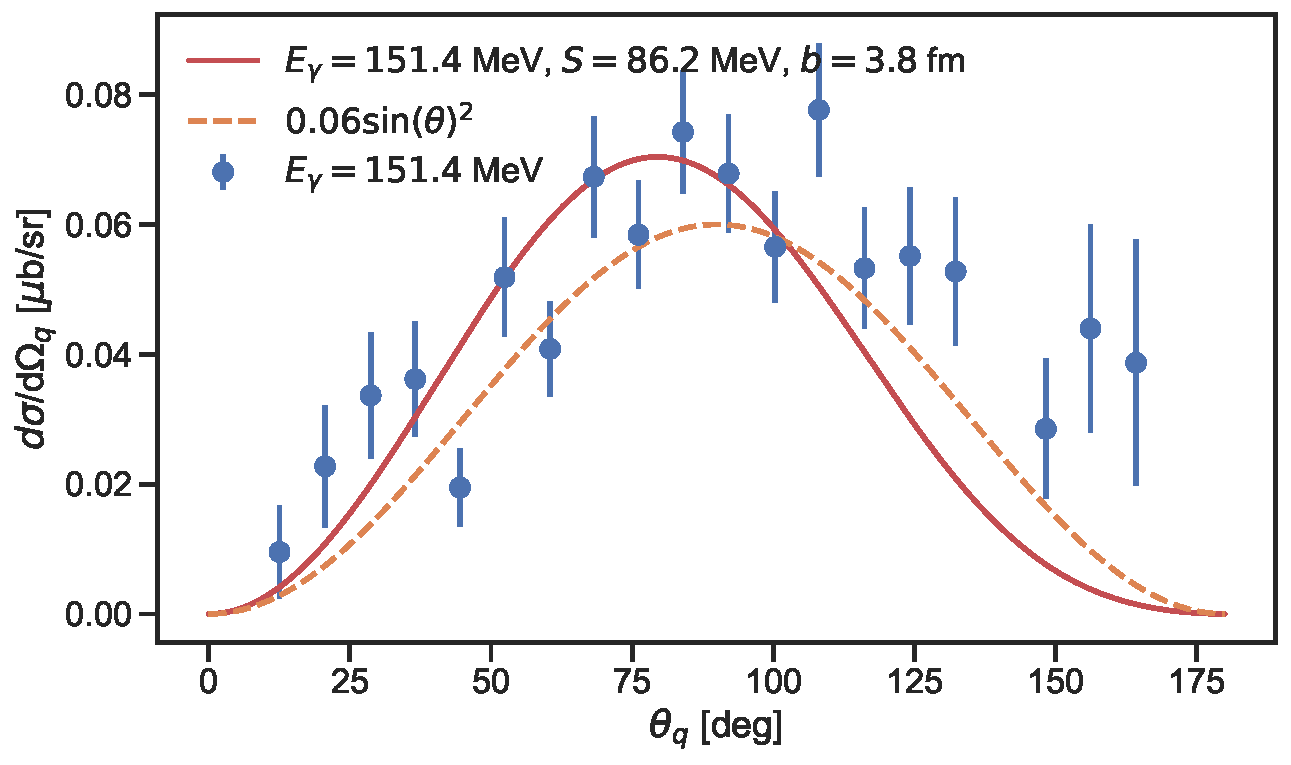
\includegraphics[width=\linewidth]{Figures/DiffCross151_rel.pdf}
	\end{sidecaption}
\end{figure}
Figure \ref{fig:angular151} also shows how the angular dependency is not proportional to $\sin(\theta_q)^2$ but also has some contribution from $F(s)$. Figure \ref{fig:MultipleEnergies} shows multiple different photon energies.
\begin{figure}[H]
	\begin{sidecaption}{Angular distribution and experimental data for three different energies. Data is from \cite{BeckPion}}[fig:MultipleEnergies]
		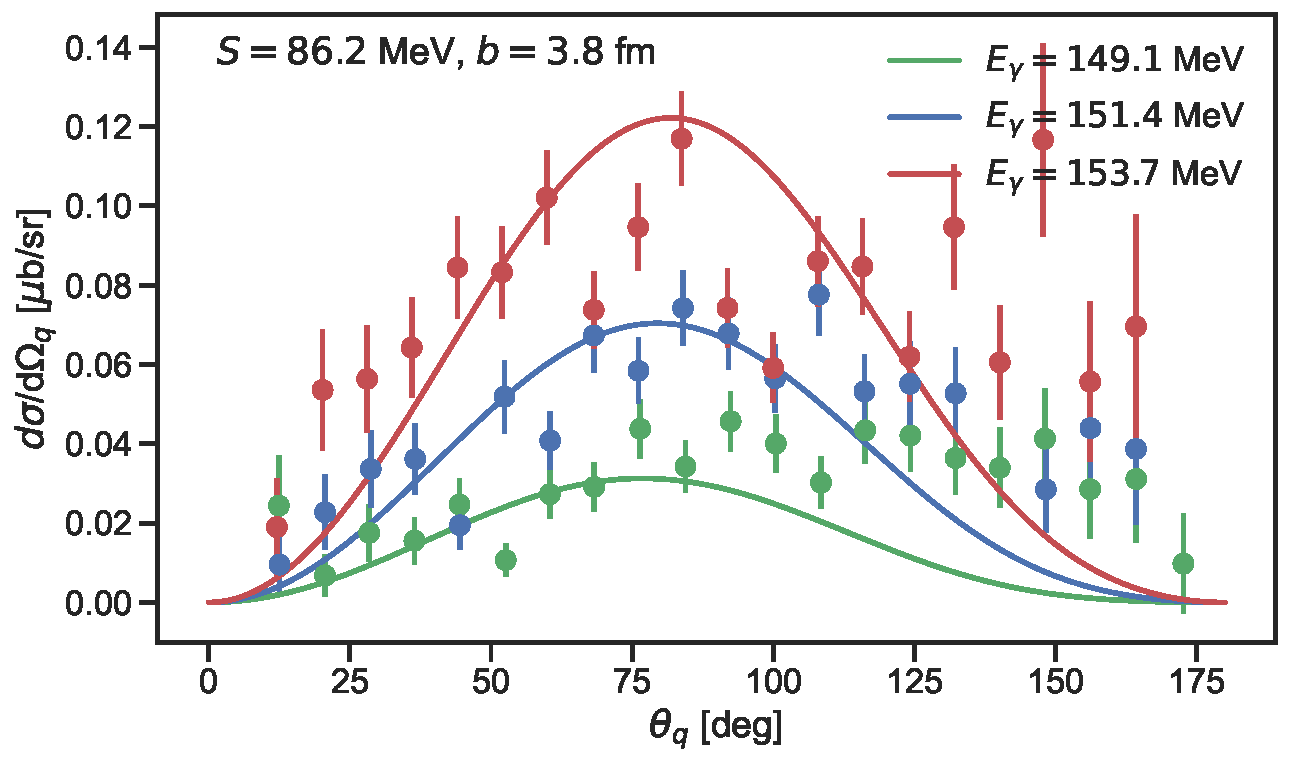
\includegraphics[width=\linewidth]{Figures/MultiDiffcross_rel.pdf}
	\end{sidecaption}
\end{figure}
Figures for the differential cross-section using different parameters and using the non-relativistic density of states are shown in appendix \ref{sec:Angular}.

The final thing we need to consider is the relative weight of the $\pi^0$ component in the wave function of the dressed proton. As in section \ref{sec:dipoleapprox}, it is expressed as 
\begin{equation}
	C(\psi_{N\pi^0})= \int_V \text{d}^3R \int_V \text{d}^3 r \, \abs{\psi_{N\pi}}^2 = 4\pi \int_0^\infty \text{d}r \, \phi(r)^2r^4
\end{equation}
For the three sets of parameters shown in figure \ref{fig:crossfitrel}, the contribution to the wave function from the $\pi^0$ is shown in figure \ref{fig:ContributionPlot}
\begin{figure}[H]
	\begin{sidecaption}{Radial wave functions using the parameters shown figure \ref{fig:crossfitrel}. Also includes virtual pions contribution to the dressed proton and the relative weight of the $\pi^0$ component in the wave function. The parameters $S,b$ match the colours from figure \ref{fig:crossfitrel}.}[fig:ContributionPlot]
		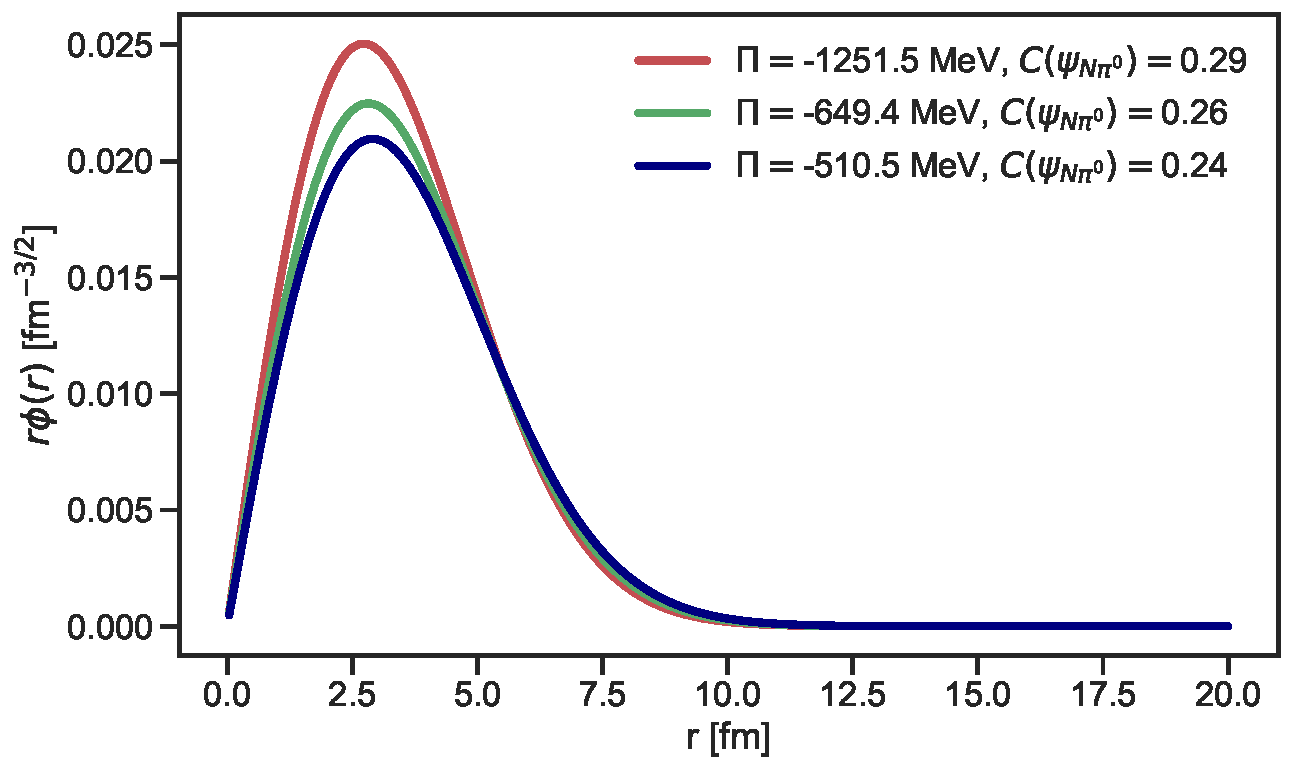
\includegraphics[width=\linewidth]{Figures/ContributionPlot.pdf} 
	\end{sidecaption}
\end{figure}
From figure \ref{fig:ContributionPlot} we see the pion-nucleon wave function constitutes about $24\%$ to $29\%$ of the total wave function. This also concludes the treatment of neutral pion photoproduction off protons. This section described the general framework of how to calculate the total cross-section and contribution from the pion-nucleon system to the total wave function. These two results are shown in figure \ref{fig:crossfitrel} and figure \ref{fig:ContributionPlot}, respectively. 
\newpage
\subsection{Neutral Pion Photoproduction off Neutrons}\label{sec:NoffN}
Having considered neutral pions off protons, we now consider the closely related neutral pions off neutrons,
\begin{equation} \label{process2}
	n\gamma \rightarrow \pi^0 n,
\end{equation}
The Feynman diagram of the equation \eqref{process2} is shown in figure \ref{Feynman2}. The key difference compared to \eqref{prod1} is that now the pion is responsible for the interaction with the electromagnetic field, and hence equation \eqref{RadiationHamil} depends on the pion, which yields the following expression
\begin{marginfigure}
	\centering
	

\tikzset{every picture/.style={line width=0.75pt}} %set default line width to 0.75pt        

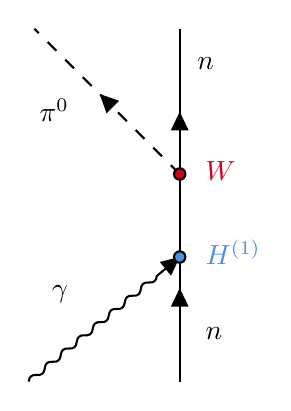
\begin{tikzpicture}[x=0.75pt,y=0.75pt,yscale=-1,xscale=1]
	%uncomment if require: \path (0,300); %set diagram left start at 0, and has height of 300
	
	%Straight Lines [id:da33488681649693186] 
	\draw    (270,210) -- (270,130) ;
	\draw [shift={(270,165)}, rotate = 90] [fill={rgb, 255:red, 0; green, 0; blue, 0 }  ][line width=0.08]  [draw opacity=0] (8.93,-4.29) -- (0,0) -- (8.93,4.29) -- cycle    ;
	%Straight Lines [id:da46389908648611555] 
	\draw    (197.25,210) .. controls (197.48,207.65) and (198.76,206.59) .. (201.11,206.82) .. controls (203.46,207.05) and (204.74,205.99) .. (204.96,203.64) .. controls (205.19,201.29) and (206.47,200.23) .. (208.82,200.46) .. controls (211.17,200.68) and (212.45,199.62) .. (212.68,197.27) .. controls (212.91,194.92) and (214.19,193.86) .. (216.54,194.09) .. controls (218.89,194.32) and (220.17,193.26) .. (220.39,190.91) .. controls (220.62,188.56) and (221.9,187.5) .. (224.25,187.73) .. controls (226.6,187.96) and (227.88,186.9) .. (228.11,184.55) .. controls (228.34,182.2) and (229.62,181.14) .. (231.97,181.37) .. controls (234.32,181.6) and (235.6,180.54) .. (235.82,178.19) .. controls (236.05,175.84) and (237.33,174.78) .. (239.68,175.01) .. controls (242.03,175.23) and (243.31,174.17) .. (243.54,171.82) .. controls (243.77,169.47) and (245.05,168.41) .. (247.4,168.64) .. controls (249.75,168.87) and (251.03,167.81) .. (251.25,165.46) .. controls (251.48,163.11) and (252.76,162.05) .. (255.11,162.28) .. controls (257.46,162.51) and (258.74,161.45) .. (258.97,159.1) -- (261.51,157) -- (267.69,151.91) ;
	\draw [shift={(270,150)}, rotate = 140.49] [fill={rgb, 255:red, 0; green, 0; blue, 0 }  ][line width=0.08]  [draw opacity=0] (8.93,-4.29) -- (0,0) -- (8.93,4.29) -- cycle    ;
	%Straight Lines [id:da3810232285211974] 
	\draw  [dash pattern={on 4.5pt off 4.5pt}]  (270,110) -- (200,40) ;
	\draw [shift={(231.46,71.46)}, rotate = 45] [fill={rgb, 255:red, 0; green, 0; blue, 0 }  ][line width=0.08]  [draw opacity=0] (8.93,-4.29) -- (0,0) -- (8.93,4.29) -- cycle    ;
	%Straight Lines [id:da6452866026111611] 
	\draw    (270,130) -- (270,40) ;
	\draw [shift={(270,80)}, rotate = 90] [fill={rgb, 255:red, 0; green, 0; blue, 0 }  ][line width=0.08]  [draw opacity=0] (8.93,-4.29) -- (0,0) -- (8.93,4.29) -- cycle    ;
	%Shape: Circle [id:dp14659197000759305] 
	\draw  [fill={rgb, 255:red, 74; green, 144; blue, 226 }  ,fill opacity=1 ] (267.25,150) .. controls (267.25,148.48) and (268.48,147.25) .. (270,147.25) .. controls (271.52,147.25) and (272.75,148.48) .. (272.75,150) .. controls (272.75,151.52) and (271.52,152.75) .. (270,152.75) .. controls (268.48,152.75) and (267.25,151.52) .. (267.25,150) -- cycle ;
	%Shape: Circle [id:dp1667146356512621] 
	\draw  [fill={rgb, 255:red, 208; green, 2; blue, 27 }  ,fill opacity=1 ] (267.25,110) .. controls (267.25,108.48) and (268.48,107.25) .. (270,107.25) .. controls (271.52,107.25) and (272.75,108.48) .. (272.75,110) .. controls (272.75,111.52) and (271.52,112.75) .. (270,112.75) .. controls (268.48,112.75) and (267.25,111.52) .. (267.25,110) -- cycle ;
	
	% Text Node
	\draw (281,182.4) node [anchor=north west][inner sep=0.75pt]    {$n$};
	% Text Node
	\draw (277,52.4) node [anchor=north west][inner sep=0.75pt]    {$n$};
	% Text Node
	\draw (201,72.4) node [anchor=north west][inner sep=0.75pt]    {$\pi ^{0}$};
	% Text Node
	\draw (207,162.4) node [anchor=north west][inner sep=0.75pt]    {$\gamma $};
	% Text Node
	\draw (281,140.4) node [anchor=north west][inner sep=0.75pt]  [color={rgb, 255:red, 74; green, 144; blue, 226 }  ,opacity=1 ]  {$H^{( 1)}$};
	% Text Node
	\draw (281,102.4) node [anchor=north west][inner sep=0.75pt]  [color={rgb, 255:red, 208; green, 2; blue, 27 }  ,opacity=1 ]  {$W$};
	
	
\end{tikzpicture}
	\caption{Feynman diagram of neutral pion photoproduction off protons. The blue vertex corresponds to equation \eqref{RadiNeutron} and the red vertex corresponds to equation \eqref{W}.}
	\label{Feynman2}
\end{marginfigure} 
\begin{equation} \label{RadiNeutron}
	H^{(1)} = -\frac{e}{m_\pi c}\vec{A}(\vec{r}_\pi,t)\cdot\vec{p}_\pi.
\end{equation}
\begin{marginfigure}
	\centering
	

\tikzset{every picture/.style={line width=0.75pt}} %set default line width to 0.75pt        

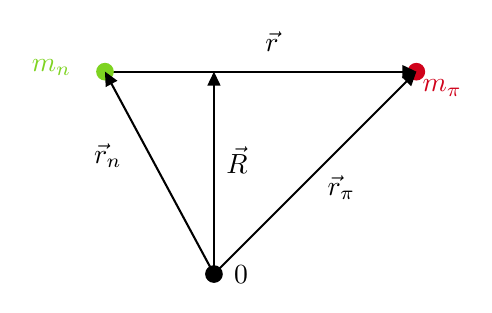
\begin{tikzpicture}[x=0.75pt,y=0.75pt,yscale=-0.75,xscale=0.75]
	%uncomment if require: \path (0,300); %set diagram left start at 0, and has height of 300
	
	%Flowchart: Connector [id:dp9827455772611288] 
	\draw  [color={rgb, 255:red, 208; green, 2; blue, 27 }  ,draw opacity=1 ][fill={rgb, 255:red, 208; green, 2; blue, 27 }  ,fill opacity=1 ] (315,90) .. controls (315,87.24) and (317.24,85) .. (320,85) .. controls (322.76,85) and (325,87.24) .. (325,90) .. controls (325,92.76) and (322.76,95) .. (320,95) .. controls (317.24,95) and (315,92.76) .. (315,90) -- cycle ;
	%Straight Lines [id:da5093684133345362] 
	\draw    (125,90) -- (317,90) ;
	\draw [shift={(320,90)}, rotate = 180] [fill={rgb, 255:red, 0; green, 0; blue, 0 }  ][line width=0.08]  [draw opacity=0] (8.93,-4.29) -- (0,0) -- (8.93,4.29) -- cycle    ;
	%Straight Lines [id:da04984112064582158] 
	\draw    (190,220) -- (190,93) ;
	\draw [shift={(190,90)}, rotate = 90] [fill={rgb, 255:red, 0; green, 0; blue, 0 }  ][line width=0.08]  [draw opacity=0] (8.93,-4.29) -- (0,0) -- (8.93,4.29) -- cycle    ;
	%Straight Lines [id:da13661676787341415] 
	\draw    (190,220) -- (317.88,92.12) ;
	\draw [shift={(320,90)}, rotate = 135] [fill={rgb, 255:red, 0; green, 0; blue, 0 }  ][line width=0.08]  [draw opacity=0] (8.93,-4.29) -- (0,0) -- (8.93,4.29) -- cycle    ;
	%Flowchart: Connector [id:dp37210275318157304] 
	\draw  [color={rgb, 255:red, 126; green, 211; blue, 33 }  ,draw opacity=1 ][fill={rgb, 255:red, 126; green, 211; blue, 33 }  ,fill opacity=1 ] (115,90) .. controls (115,87.24) and (117.24,85) .. (120,85) .. controls (122.76,85) and (125,87.24) .. (125,90) .. controls (125,92.76) and (122.76,95) .. (120,95) .. controls (117.24,95) and (115,92.76) .. (115,90) -- cycle ;
	%Straight Lines [id:da8769015497622031] 
	\draw    (190,220) -- (121.42,92.64) ;
	\draw [shift={(120,90)}, rotate = 61.7] [fill={rgb, 255:red, 0; green, 0; blue, 0 }  ][line width=0.08]  [draw opacity=0] (8.93,-4.29) -- (0,0) -- (8.93,4.29) -- cycle    ;
	%Flowchart: Connector [id:dp5562170943538245] 
	\draw  [color={rgb, 255:red, 0; green, 0; blue, 0 }  ,draw opacity=1 ][fill={rgb, 255:red, 0; green, 0; blue, 0 }  ,fill opacity=1 ] (185,220) .. controls (185,217.24) and (187.24,215) .. (190,215) .. controls (192.76,215) and (195,217.24) .. (195,220) .. controls (195,222.76) and (192.76,225) .. (190,225) .. controls (187.24,225) and (185,222.76) .. (185,220) -- cycle ;
	
	% Text Node
	\draw (71,80.4) node [anchor=north west][inner sep=0.75pt]  [color={rgb, 255:red, 126; green, 211; blue, 33 }  ,opacity=1 ]  {$m_{n}$};
	% Text Node
	\draw (322,93.4) node [anchor=north west][inner sep=0.75pt]  [color={rgb, 255:red, 208; green, 2; blue, 27 }  ,opacity=1 ]  {$m_{\pi }$};
	% Text Node
	\draw (196,136.4) node [anchor=north west][inner sep=0.75pt]    {$\vec{R}$};
	% Text Node
	\draw (261,155) node [anchor=north west][inner sep=0.75pt]    {$\vec{r}_{\pi }$};
	% Text Node
	\draw (111,134.4) node [anchor=north west][inner sep=0.75pt]    {$\vec{r}_{n}$};
	% Text Node
	\draw (221,62.4) node [anchor=north west][inner sep=0.75pt]    {$\vec{r}$};
	% Text Node
	\draw (201,212.4) node [anchor=north west][inner sep=0.75pt]    {$0$};
	
	
\end{tikzpicture}
	\caption{Sketch of the system. Here $\vec{r}_n$ is the coordinate of the proton and $\vec{r}_\pi$ is the coordinate of the pion. The relative coordinate is given by $\vec{r}=\vec{r}_\pi-\vec{r}_n$ and the coordinate of the center-of-mass is $\vec{R}=(m_n \vec{r}_n+m_\pi\vec{r}_\pi)/(m_n+m_\pi)$. The total mass is denoted $M_{n\pi}=m_n+m_\pi$.}
	\label{JacobiIllustrationNeutron}
\end{marginfigure}
This changes two things in comparison to equation \eqref{exactdiffcross}. The mass of the proton becomes the mass of the pion, and the wave number vector becomes $\vec{s}=\vec{q}-\frac{m_n}{M_{n\pi}}\vec{k}$, where $m_n$ is the mass of the neutron. Therefore the final expression for the differential cross-section using the relativistic density of states 
\begin{equation} \label{totalcrossneutron}
	\frac{\text{d}\sigma^0(E_q,\theta_q)}{\text{d}\Omega_q} = \frac{e^2}{8\pi}\frac{1}{m_\pi^2c^4}\frac{q^3}{k}\frac{\text{d}(\hbar c q)^2}{\text{d}E_q}\sin^2(\theta_q) s^2 F(s)^2.
\end{equation}
This leads to the following expression for the total cross-section
\begin{equation} \label{pionneutraloffneutron}
	\sigma^0 = 2\pi \int_0^\pi \text{d}\theta_q \, \frac{e^2}{8\pi}\frac{1}{m_\pi^2c^4}\frac{q^3}{k}\frac{\text{d}(\hbar c q)^2}{\text{d}E_q}\sin^2(\theta_q) s^3 F(s)^2.
\end{equation}
Unfortunately, no experimental data exists such that a fit can be performed. Due to the similarities between the proton and the neutron, one could expect experimental data similar to figure \ref{fig:crossfitrel}, which would mean different fit parameters since the pion is now responsible for the interaction with the electromagnetic field. Figure \ref{fig:neutralpionsoffneutrons} shows the total cross-section for the process in equation \eqref{process2} using the same fit parameters as in the previous section. The dashed lines represent the non-relativistic density of states which yields the following 
\begin{equation} \label{nonrelcrossfitneutron}
	\sigma^0 = 2\pi \int_0^\pi \text{d}\theta_q \, \frac{e^2}{4\pi}\frac{\mu_{n\pi}c^2}{m_\pi^2 c^4}\frac{q^3}{k}\sin^3(\theta_q)s^2 F(s)^2.
\end{equation} 
\begin{figure}[H]
	\begin{sidecaption}{The process $\gamma n \rightarrow \pi^0 n$ with the same parameters as for neutral pion photoproduction off protons. The dashed lines represent the non-relativistic density of states \eqref{nonrelcrossfitneutron}. The threshold energy for this process is 144.7 MeV.}[fig:neutralpionsoffneutrons]
		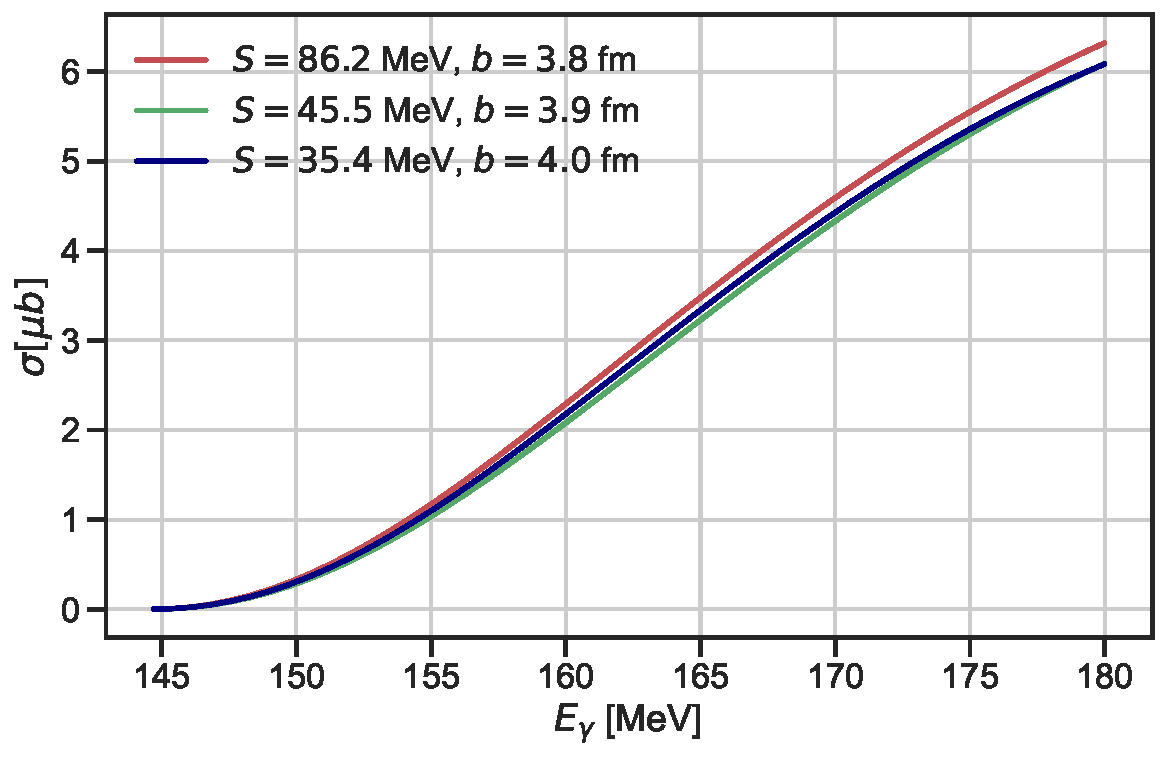
\includegraphics[width=\linewidth]{Figures/NeutralPionsOffNeutrons.pdf}
	\end{sidecaption}
\end{figure}
Note that the relative weight from the pion-nucleon channel will be identical to figure \ref{fig:ContributionPlot} since these only depend on the parameters $S,b$. 
\subsection{Charged Pion Photoproduction off Protons}\label{sec:CoffP}
Moving on to charged pions, we first consider the following process,
\begin{equation} \label{charged1}
	p\gamma \rightarrow \pi^+ n,
\end{equation}
where charged pions are generated off the proton. Note that the charged pion is different in two ways compared to the neutral pion. The mass is approximately $5$ MeV higher, and it contains an isospin coefficient from \eqref{isocoeff}, which means we get the following extra contribution
\begin{equation} \label{isofactorcharged}
	\mel*{n\pi^+}{\vec{\tau}\cdot\vec{\pi}}{p} = \sqrt{2}.
\end{equation}
Carrying this factor through the derivations in section \ref{sec:NeutralOffProton} amounts to a factor of 2. This means the total cross-section is given by
\begin{marginfigure}
	\centering
	

\tikzset{every picture/.style={line width=0.75pt}} %set default line width to 0.75pt        

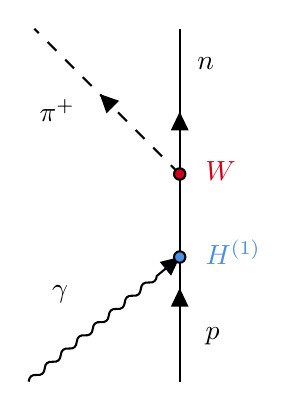
\begin{tikzpicture}[x=0.75pt,y=0.75pt,yscale=-1,xscale=1]
	%uncomment if require: \path (0,300); %set diagram left start at 0, and has height of 300
	
	%Straight Lines [id:da33488681649693186] 
	\draw    (270,210) -- (270,130) ;
	\draw [shift={(270,165)}, rotate = 90] [fill={rgb, 255:red, 0; green, 0; blue, 0 }  ][line width=0.08]  [draw opacity=0] (8.93,-4.29) -- (0,0) -- (8.93,4.29) -- cycle    ;
	%Straight Lines [id:da46389908648611555] 
	\draw    (197.25,210) .. controls (197.48,207.65) and (198.76,206.59) .. (201.11,206.82) .. controls (203.46,207.05) and (204.74,205.99) .. (204.96,203.64) .. controls (205.19,201.29) and (206.47,200.23) .. (208.82,200.46) .. controls (211.17,200.68) and (212.45,199.62) .. (212.68,197.27) .. controls (212.91,194.92) and (214.19,193.86) .. (216.54,194.09) .. controls (218.89,194.32) and (220.17,193.26) .. (220.39,190.91) .. controls (220.62,188.56) and (221.9,187.5) .. (224.25,187.73) .. controls (226.6,187.96) and (227.88,186.9) .. (228.11,184.55) .. controls (228.34,182.2) and (229.62,181.14) .. (231.97,181.37) .. controls (234.32,181.6) and (235.6,180.54) .. (235.82,178.19) .. controls (236.05,175.84) and (237.33,174.78) .. (239.68,175.01) .. controls (242.03,175.23) and (243.31,174.17) .. (243.54,171.82) .. controls (243.77,169.47) and (245.05,168.41) .. (247.4,168.64) .. controls (249.75,168.87) and (251.03,167.81) .. (251.25,165.46) .. controls (251.48,163.11) and (252.76,162.05) .. (255.11,162.28) .. controls (257.46,162.51) and (258.74,161.45) .. (258.97,159.1) -- (261.51,157) -- (267.69,151.91) ;
	\draw [shift={(270,150)}, rotate = 140.49] [fill={rgb, 255:red, 0; green, 0; blue, 0 }  ][line width=0.08]  [draw opacity=0] (8.93,-4.29) -- (0,0) -- (8.93,4.29) -- cycle    ;
	%Straight Lines [id:da3810232285211974] 
	\draw  [dash pattern={on 4.5pt off 4.5pt}]  (270,110) -- (200,40) ;
	\draw [shift={(231.46,71.46)}, rotate = 45] [fill={rgb, 255:red, 0; green, 0; blue, 0 }  ][line width=0.08]  [draw opacity=0] (8.93,-4.29) -- (0,0) -- (8.93,4.29) -- cycle    ;
	%Straight Lines [id:da6452866026111611] 
	\draw    (270,130) -- (270,40) ;
	\draw [shift={(270,80)}, rotate = 90] [fill={rgb, 255:red, 0; green, 0; blue, 0 }  ][line width=0.08]  [draw opacity=0] (8.93,-4.29) -- (0,0) -- (8.93,4.29) -- cycle    ;
	%Shape: Circle [id:dp14659197000759305] 
	\draw  [fill={rgb, 255:red, 74; green, 144; blue, 226 }  ,fill opacity=1 ] (267.25,150) .. controls (267.25,148.48) and (268.48,147.25) .. (270,147.25) .. controls (271.52,147.25) and (272.75,148.48) .. (272.75,150) .. controls (272.75,151.52) and (271.52,152.75) .. (270,152.75) .. controls (268.48,152.75) and (267.25,151.52) .. (267.25,150) -- cycle ;
	%Shape: Circle [id:dp1667146356512621] 
	\draw  [fill={rgb, 255:red, 208; green, 2; blue, 27 }  ,fill opacity=1 ] (267.25,110) .. controls (267.25,108.48) and (268.48,107.25) .. (270,107.25) .. controls (271.52,107.25) and (272.75,108.48) .. (272.75,110) .. controls (272.75,111.52) and (271.52,112.75) .. (270,112.75) .. controls (268.48,112.75) and (267.25,111.52) .. (267.25,110) -- cycle ;
	
	% Text Node
	\draw (281,182.4) node [anchor=north west][inner sep=0.75pt]    {$p$};
	% Text Node
	\draw (277,52.4) node [anchor=north west][inner sep=0.75pt]    {$n$};
	% Text Node
	\draw (201,72.4) node [anchor=north west][inner sep=0.75pt]    {$\pi ^{+}$};
	% Text Node
	\draw (207,162.4) node [anchor=north west][inner sep=0.75pt]    {$\gamma $};
	% Text Node
	\draw (281,140.4) node [anchor=north west][inner sep=0.75pt]  [color={rgb, 255:red, 74; green, 144; blue, 226 }  ,opacity=1 ]  {$H^{( 1)}$};
	% Text Node
	\draw (281,102.4) node [anchor=north west][inner sep=0.75pt]  [color={rgb, 255:red, 208; green, 2; blue, 27 }  ,opacity=1 ]  {$W$};
	
	
\end{tikzpicture}
	\caption{Feynman diagram of neutral pion photoproduction off protons. The blue vertex corresponds to equation \eqref{1trans} and the red vertex corresponds to equation \eqref{W}.}
	\label{Feynman3}
\end{marginfigure} 
\begin{equation} \label{totcross3}
	\sigma^+ =  2\pi \int_0^\pi \text{d}\theta_q \, \frac{e^2}{4\pi}\frac{1}{m_p^2c^4}\frac{q^3}{k}\frac{\text{d}(\hbar c q)^2}{\text{d}E_q}\sin^3(\theta_q) s^2 F(s)^2,
\end{equation}
where the $+$ indicates the production of positively charged pions. Using the non-relativistic density of states, the total cross-section can be written as
\begin{equation} \label{totcross3nonrel}
	\sigma^+ =  2\pi \int_0^\pi \text{d}\theta_q \, \frac{e^2}{2\pi}\frac{\mu_{p\pi}c^2}{m_p^2c^4}\frac{q^3}{k}\sin^3(\theta_q) s^2 F(s)^2,
\end{equation}
We once again fit equation \eqref{totcross3} to experimental data from \cite{PionOffNeutron}. The result can be seen in figure \ref{fig:ChargedPionOffProton}.
\begin{figure}[H]
	\begin{sidecaption}{Fitted parameters for the process $p\gamma \rightarrow n\pi^+$. The parameters are shown inside the figure. The dashed lines represent the non-relativistic density of states \eqref{totcross3nonrel}. Data from \cite{PionOffNeutron}. The threshold energy for this process is 151.4 MeV.}[fig:ChargedPionOffProton]
		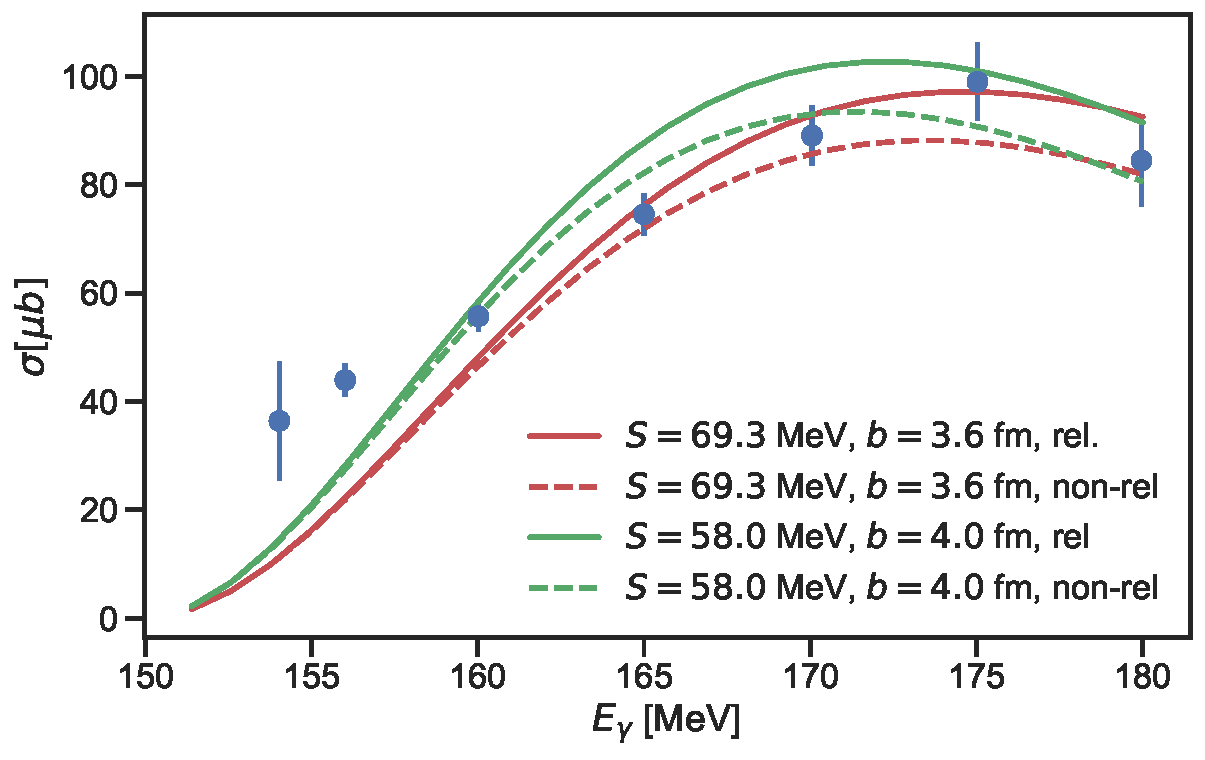
\includegraphics[width=\linewidth]{Figures/ChargedPionOffProtonExact_fitted.pdf}
	\end{sidecaption}
\end{figure}
Figure \ref{fig:ChargedPionOffProton} shows the model has difficulty accurately describing the pion photoproduction of charged pions. The data points near the threshold cannot adequately be described by the parameters shown in the figure. This can be explained by the spherical Bessel function $j_1(sr)$ in the integral $F(s)$ in equation \eqref{totcross3}. The spherical Bessel function is 0 for $s=0$, which means the data points near the threshold can only be included if the integral increases rapidly intermediately after the threshold. There is a trade-off since the $r^3$ dependency begins to dominate the integral. This means the data points near the threshold can be better described by the $j_0(qr)$ as in the dipole approximation. A combined plot is shown in figure \ref{fig:CombinedPlot}. 
\newpage
\begin{figure}[H]
	\begin{sidecaption}{Best fit using both the dipole approximation for data points near the threshold and the exact approach for energies where the dipole approximation is no longer valid.}[fig:CombinedPlot]
		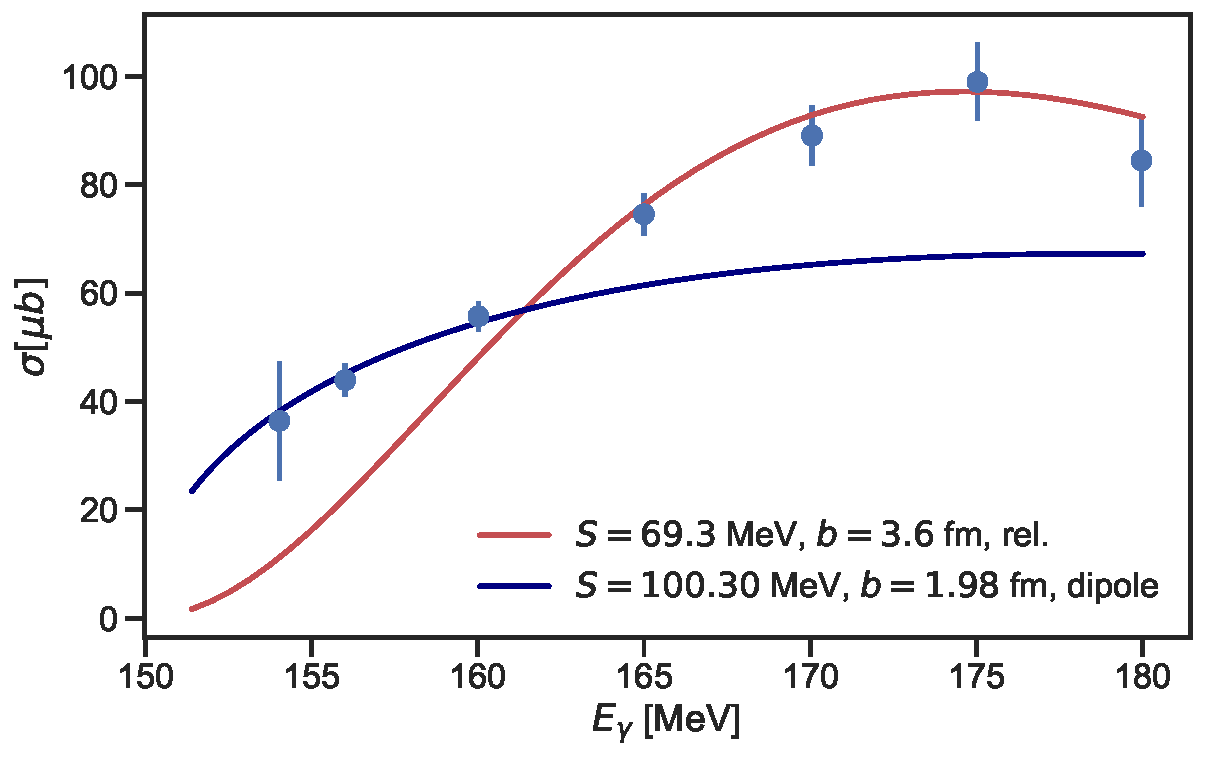
\includegraphics[width=\linewidth]{Figures/ChargedPionOffProtonExact1.pdf}
	\end{sidecaption}
\end{figure}
We now focus on the weight of the $\pi^+$ component in the wave function and the pions contribution to the mass of the dressed proton. This is shown in figure \ref{fig:ContributionPlotPlus} where the colours match from figure \ref{fig:ChargedPionOffProton} and figure \ref{fig:CombinedPlot}.
\begin{figure}[H]
	\begin{sidecaption}{Radial wave functions using the parameters shown figure \ref{fig:ChargedPionOffProton} and figure \ref{fig:CombinedPlot}. Also includes virtual pions contribution to the dressed proton and the relative weight of the $\pi^+$ component in the wave function.}[fig:ContributionPlotPlus]
		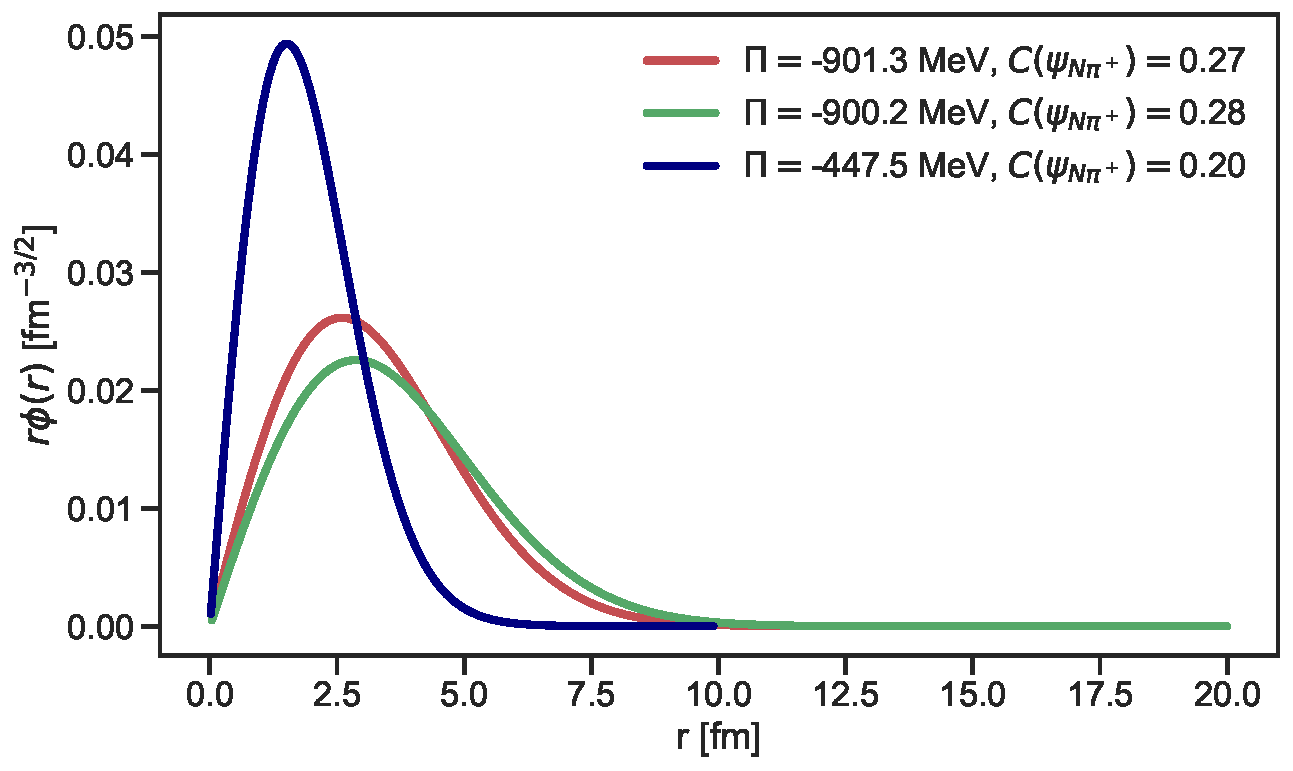
\includegraphics[width=\linewidth]{Figures/ContributionPlotPiPlus.pdf}
	\end{sidecaption}
\end{figure}
The energy is much lower when considering the parameters from the dipole approximation. The contributions are similar, which is impressive considering a difference of $S \sim  40$ MeV and $b\sim2$ fm in the parameters. 

The cross-section is one observable, which is related to how much the pion-nucleon wave function contributes to the total wave function, as shown in figure  \ref{fig:ContributionPlotPlus}. From the formalism described in section \ref{Decsofmodel} we can relate this to another observable, the charge density. We restrict the results to only consider charged pions since there is no experimental data for the process mentioned in section \ref{sec:CoffP} and hence no set of parameters $S,b$. The two-component wave function contains the wave function $\psi_{N\pi}(\vec{r}_\pi,\vec{r}_N)$, which is a two-dimensional position wave function. This is means the probability density in a volume $\text{d}\vec{r}_\pi \, \text{d}\vec{r}_p$ at position $(\vec{r}_\pi,\vec{r}_p)$ is given by
\begin{equation}\label{probdens}
	\rho(\vec{r}_\pi,\vec{r}_p) = \abs{\psi_{N\pi}(\vec{r}_\pi,\vec{r}_p)}^2,
\end{equation}
and the probability of finding the pion at position $\vec{r}_\pi$ is then
\begin{equation}\label{posirpi}
	\rho_\pi(\vec{r}_\pi) = \int \text{d}\vec{r}_p \abs{\psi(\vec{r}_\pi,\vec{r}_p)}^2,
\end{equation}
where we now omit the index and remind ourselves that the radial wave function is given by $\psi=r\phi$ from section \ref{sec:numericalconsiderations}. This leads to the following expression for the total charge density of the pion-nucleon system
\begin{equation}\label{pionnuccharge}
	\rho(\vec{r}) = q_\pi \int \text{d}\vec{r}_\pi \text{d}\vec{r}_p \, \abs{\psi(\vec{r}_\pi,\vec{r}_p)}^2+q_p \int \text{d}\vec{r}_\pi \text{d}\vec{r}_p \, \abs{\psi(\vec{r}_\pi,\vec{r}_p)}^2,
\end{equation}
where $q_\pi$ and $q_p$ are the charge of the pion and the proton, respectively. We now compute the two integrals in the center of mass using the relative coordinates illustrated in figure \ref{JacobiIllustration}.
\begin{align}
	\rho_\pi(\vec{r}_\text{cm}) &= q_\pi \int \text{d}\vec{r}_\pi \text{d} \vec{r}_p \, \abs{\psi(\vec{r}_\pi,\vec{r}_p)}^2 \delta(\vec{r_\pi-\vec{R}},\vec{r}_\text{cm}) \\
	&= q_\pi \int \text{d}\vec{r} \,\text{d}\vec{R} \, \bigg\lvert\vec{r}\phi\bigg(\vec{R}+\frac{m_p}{M_{p\pi}}\vec{r},\vec{R}-\frac{m_\pi}{M_{p\pi}}\bigg)\bigg\rvert^2 \delta(\vec{R}+\frac{m_p}{M_{p\pi}}\vec{r}-\vec{R},\vec{r}_\text{cm}) \\
	&= q_\pi \bigg \lvert\frac{M_{p\pi}}{m_p}\vec{r}_\text{cm}\phi\bigg(\frac{M_{p\pi}}{m_p}\vec{r}_{\text{cm}}\bigg) \bigg\rvert^2.
\end{align}
The charge density of the nucleon can be computed in a similar manner. This means we can plot equation \eqref{pionnuccharge}, which is shown in figure \ref{fig:chargedensity} as a function of the absolute radius from the center of mass. 
\begin{figure}[H]
	\begin{sidecaption}{Charge density for the parameters $S=63.3$ MeV and $b=3.6$ fm. The charge density is normalised in such a way that the total charge $Q$ is unity.}[fig:chargedensity]
		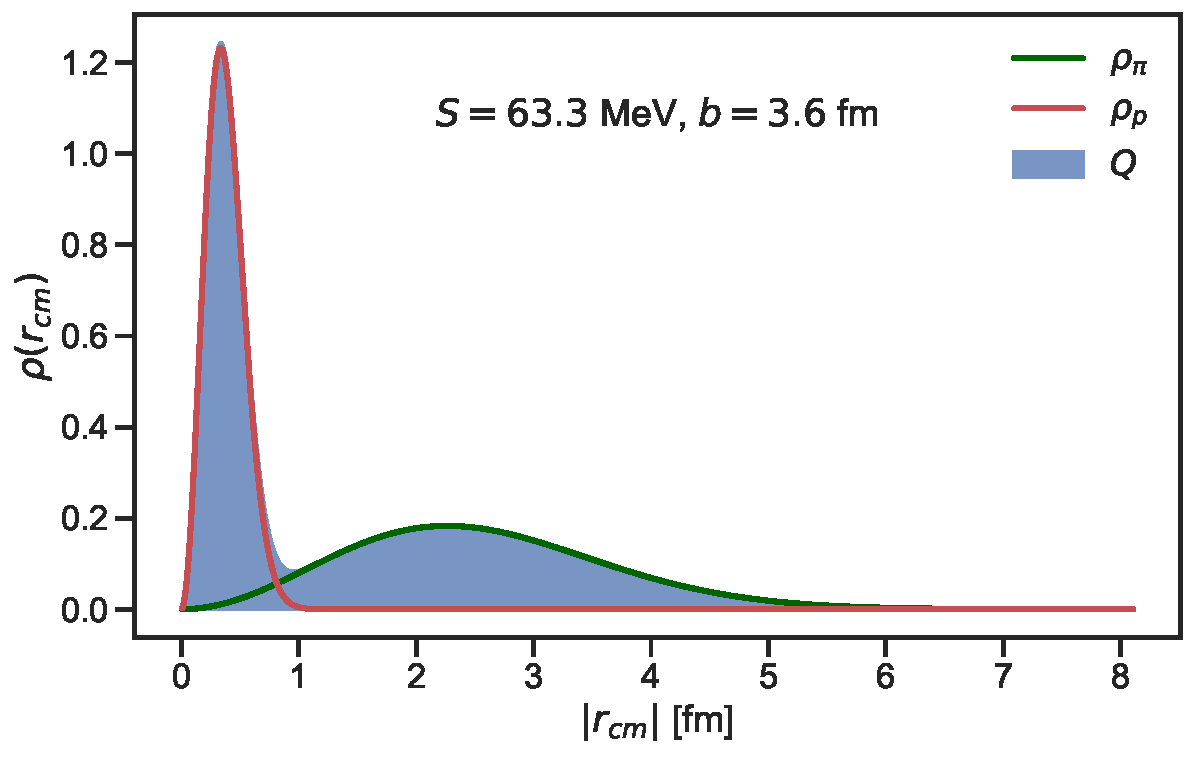
\includegraphics[width=\linewidth]{Figures/ChargeDensityNeutronPlus1.pdf} 
	\end{sidecaption}
\end{figure}
And similarly for the parameters using the dipole approximation
\begin{figure}[H]
	\begin{sidecaption}{Charge density for the parameters $S=100.30$ MeV and $b=1.98$ fm. The charge density is normalised in such a way that the total charge $Q$ is unity.}[fig:chargedensity1]
		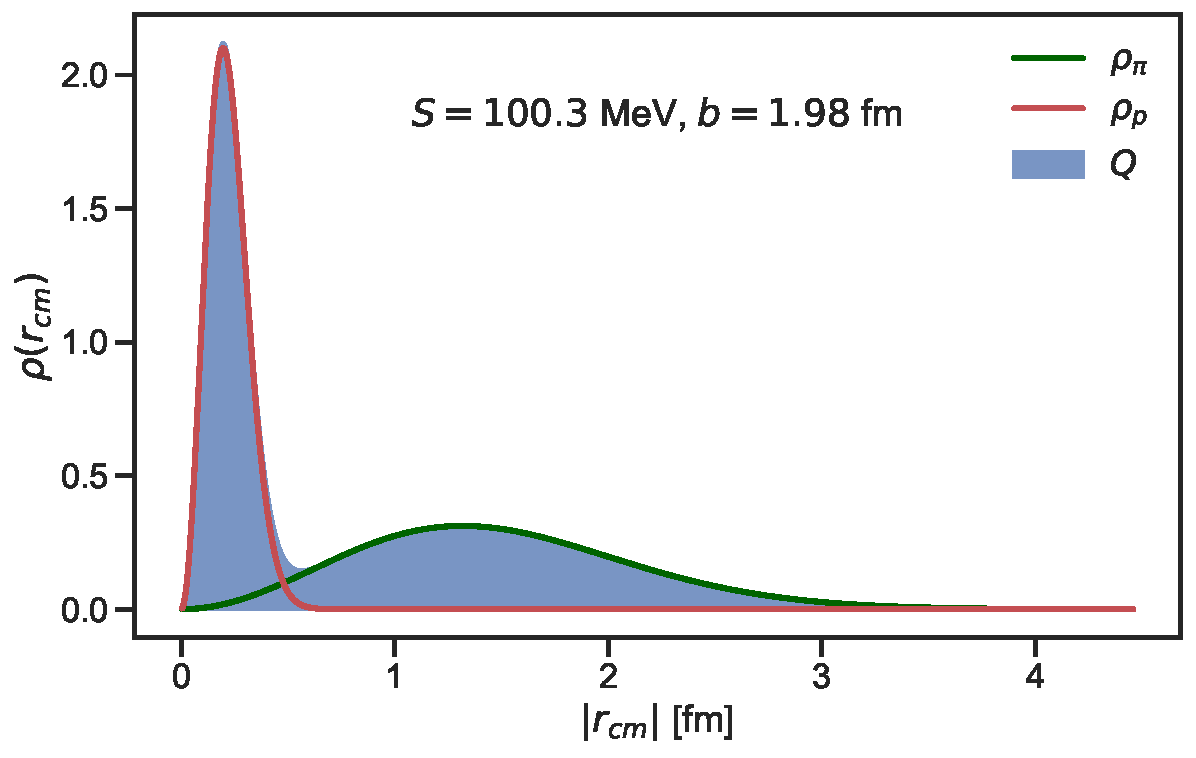
\includegraphics[width=\linewidth]{Figures/ChargeDensityNeutronPlus2.pdf} 
	\end{sidecaption}
\end{figure}
To complete the picture using the two-component wave function \eqref{superposition}, we can imagine the bare proton as a delta function at $\vec{r}_\text{cm}=0$ and the probability density of the proton in the pion-nucleon system moved a distance to the left on the figure \ref{fig:chargedensity}. The distance corresponds to the distance away from the center of mass due to the mass difference between the proton and the pion. 

\subsection{Charged Pion Photoproduction off Neutrons}\label{sec:chargedofne}
The last process to be investigated involves charged pions off a neutron,
\begin{equation} \label{proc4}
	n\gamma \rightarrow \pi^- p,
\end{equation}
which is also the most complicated since there is a Coulomb interaction between the two particles. 
\begin{marginfigure}
	\centering
	

\tikzset{every picture/.style={line width=0.75pt}} %set default line width to 0.75pt        

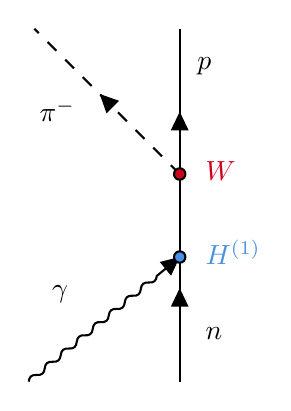
\begin{tikzpicture}[x=0.75pt,y=0.75pt,yscale=-1,xscale=1]
	%uncomment if require: \path (0,300); %set diagram left start at 0, and has height of 300
	
	%Straight Lines [id:da33488681649693186] 
	\draw    (270,210) -- (270,130) ;
	\draw [shift={(270,165)}, rotate = 90] [fill={rgb, 255:red, 0; green, 0; blue, 0 }  ][line width=0.08]  [draw opacity=0] (8.93,-4.29) -- (0,0) -- (8.93,4.29) -- cycle    ;
	%Straight Lines [id:da46389908648611555] 
	\draw    (197.25,210) .. controls (197.48,207.65) and (198.76,206.59) .. (201.11,206.82) .. controls (203.46,207.05) and (204.74,205.99) .. (204.96,203.64) .. controls (205.19,201.29) and (206.47,200.23) .. (208.82,200.46) .. controls (211.17,200.68) and (212.45,199.62) .. (212.68,197.27) .. controls (212.91,194.92) and (214.19,193.86) .. (216.54,194.09) .. controls (218.89,194.32) and (220.17,193.26) .. (220.39,190.91) .. controls (220.62,188.56) and (221.9,187.5) .. (224.25,187.73) .. controls (226.6,187.96) and (227.88,186.9) .. (228.11,184.55) .. controls (228.34,182.2) and (229.62,181.14) .. (231.97,181.37) .. controls (234.32,181.6) and (235.6,180.54) .. (235.82,178.19) .. controls (236.05,175.84) and (237.33,174.78) .. (239.68,175.01) .. controls (242.03,175.23) and (243.31,174.17) .. (243.54,171.82) .. controls (243.77,169.47) and (245.05,168.41) .. (247.4,168.64) .. controls (249.75,168.87) and (251.03,167.81) .. (251.25,165.46) .. controls (251.48,163.11) and (252.76,162.05) .. (255.11,162.28) .. controls (257.46,162.51) and (258.74,161.45) .. (258.97,159.1) -- (261.51,157) -- (267.69,151.91) ;
	\draw [shift={(270,150)}, rotate = 140.49] [fill={rgb, 255:red, 0; green, 0; blue, 0 }  ][line width=0.08]  [draw opacity=0] (8.93,-4.29) -- (0,0) -- (8.93,4.29) -- cycle    ;
	%Straight Lines [id:da3810232285211974] 
	\draw  [dash pattern={on 4.5pt off 4.5pt}]  (270,110) -- (200,40) ;
	\draw [shift={(231.46,71.46)}, rotate = 45] [fill={rgb, 255:red, 0; green, 0; blue, 0 }  ][line width=0.08]  [draw opacity=0] (8.93,-4.29) -- (0,0) -- (8.93,4.29) -- cycle    ;
	%Straight Lines [id:da6452866026111611] 
	\draw    (270,130) -- (270,40) ;
	\draw [shift={(270,80)}, rotate = 90] [fill={rgb, 255:red, 0; green, 0; blue, 0 }  ][line width=0.08]  [draw opacity=0] (8.93,-4.29) -- (0,0) -- (8.93,4.29) -- cycle    ;
	%Shape: Circle [id:dp14659197000759305] 
	\draw  [fill={rgb, 255:red, 74; green, 144; blue, 226 }  ,fill opacity=1 ] (267.25,150) .. controls (267.25,148.48) and (268.48,147.25) .. (270,147.25) .. controls (271.52,147.25) and (272.75,148.48) .. (272.75,150) .. controls (272.75,151.52) and (271.52,152.75) .. (270,152.75) .. controls (268.48,152.75) and (267.25,151.52) .. (267.25,150) -- cycle ;
	%Shape: Circle [id:dp1667146356512621] 
	\draw  [fill={rgb, 255:red, 208; green, 2; blue, 27 }  ,fill opacity=1 ] (267.25,110) .. controls (267.25,108.48) and (268.48,107.25) .. (270,107.25) .. controls (271.52,107.25) and (272.75,108.48) .. (272.75,110) .. controls (272.75,111.52) and (271.52,112.75) .. (270,112.75) .. controls (268.48,112.75) and (267.25,111.52) .. (267.25,110) -- cycle ;
	
	% Text Node
	\draw (281,182.4) node [anchor=north west][inner sep=0.75pt]    {$n$};
	% Text Node
	\draw (277,52.4) node [anchor=north west][inner sep=0.75pt]    {$p$};
	% Text Node
	\draw (201,72.4) node [anchor=north west][inner sep=0.75pt]    {$\pi ^{-}$};
	% Text Node
	\draw (207,162.4) node [anchor=north west][inner sep=0.75pt]    {$\gamma $};
	% Text Node
	\draw (281,140.4) node [anchor=north west][inner sep=0.75pt]  [color={rgb, 255:red, 74; green, 144; blue, 226 }  ,opacity=1 ]  {$H^{( 1)}$};
	% Text Node
	\draw (281,102.4) node [anchor=north west][inner sep=0.75pt]  [color={rgb, 255:red, 208; green, 2; blue, 27 }  ,opacity=1 ]  {$W$};
	
	
\end{tikzpicture}
	\caption{Feynman diagram of neutral pion photoproduction off protons. The blue vertex corresponds to equation \eqref{RadiNeutron} and the red vertex corresponds to equation \eqref{W}.}
	\label{Feynman4}
\end{marginfigure} 
Firstly, we have to consider the dressed neutron. We can apply the same approach as we did for the dressing of the proton, but we have to include a channel where Coulomb interactions are taken into account\footnote{This is done in appendix \ref{ThreeComponentWavefunction}.}. Secondly, in the final state, we cannot use the same expansion \eqref{sphericalbesseldecomp} as we did on the plane waves. 
Ignoring this temporarily and we can deduce the expression for the total cross-section by combining the effects from section \ref{sec:NoffN} and section \ref{sec:CoffP}. This means an isospin coefficient from

\begin{equation} \label{isoceffigen}
	\mel*{p\pi^-}{\vec{\tau}\cdot\vec{\pi}}{n} = \sqrt{2},
\end{equation}
and the mass of the pion in the denominator since the pion is responsible for the interaction with the electromagnetic field. Therefore the total cross-section is given by
\begin{equation} \label{totcross4}
	\sigma^- =  2\pi \int_0^\pi \text{d}\theta_q \, \frac{e^2}{4\pi}\frac{1}{m_\pi^2c^4}\frac{q^3}{k}\frac{\text{d}(\hbar c q)^2}{\text{d}E_q}\sin^3(\theta_q) s^2 F(s)^2.
\end{equation}
However, the integral $F(s)$ is different since we have to account for the Coulomb interaction between the two charged particles in the final state. The behaviour of the charged particles can be described by an attractive Coulomb	wave function\footnote{This is covered in appendix \ref{sec:Coulomb}.}, $F_1(\eta, sr)$. This leads to the final expression for the total cross-section using the regular Coulomb wave functions
\begin{equation} \label{totcross5}
	\sigma^- =  \int_0^\pi \text{d}\theta_q \, \frac{e^2}{2}\frac{1}{m_\pi^2c^4}\frac{q^3}{k}\frac{\text{d}(\hbar c q)^2}{\text{d}E_q}\sin^3(\theta_q) s^2 \bigg(\frac{4\pi}{s} \int_0^\infty \text{d}r \, F_1(\eta,sr)r^3\phi(r)\bigg)^2,
\end{equation}
where $\eta$ is the parameter that determines the strength of the Coulomb interaction given by
\begin{equation} \label{etafunc}
	\eta = \frac{Z\mu_{p\pi}c\alpha}{\hbar k}.
\end{equation}
Here $Z$ is the product of the charges. Using the non-relativistic density of states, the expression for the total cross becomes
\begin{equation} \label{cross4nonrel}
	\sigma^-=  2\pi \int_0^\pi \text{d}\theta_q \, \frac{e^2}{2\pi}\frac{\mu_{n\pi}c^2}{m_\pi^2c^4}\frac{q^3}{k}\sin^3(\theta_q) s^2 \bigg(\frac{4\pi}{s} \int_0^\infty \text{d}r \, F_1(\eta,sr)r^3\phi(r)\bigg)^2,
\end{equation}
The fit is performed, and the results can be seen in figure \ref{fig:ChargedPionsOffNeutrons}. Data is from \cite{PionOffNeutron}.
\begin{figure}[H]
	\begin{sidecaption}{FFit of equation \eqref{totcross4} to experimental data from \cite{PionOffNeutron}.}[fig:ChargedPionsOffNeutrons]
		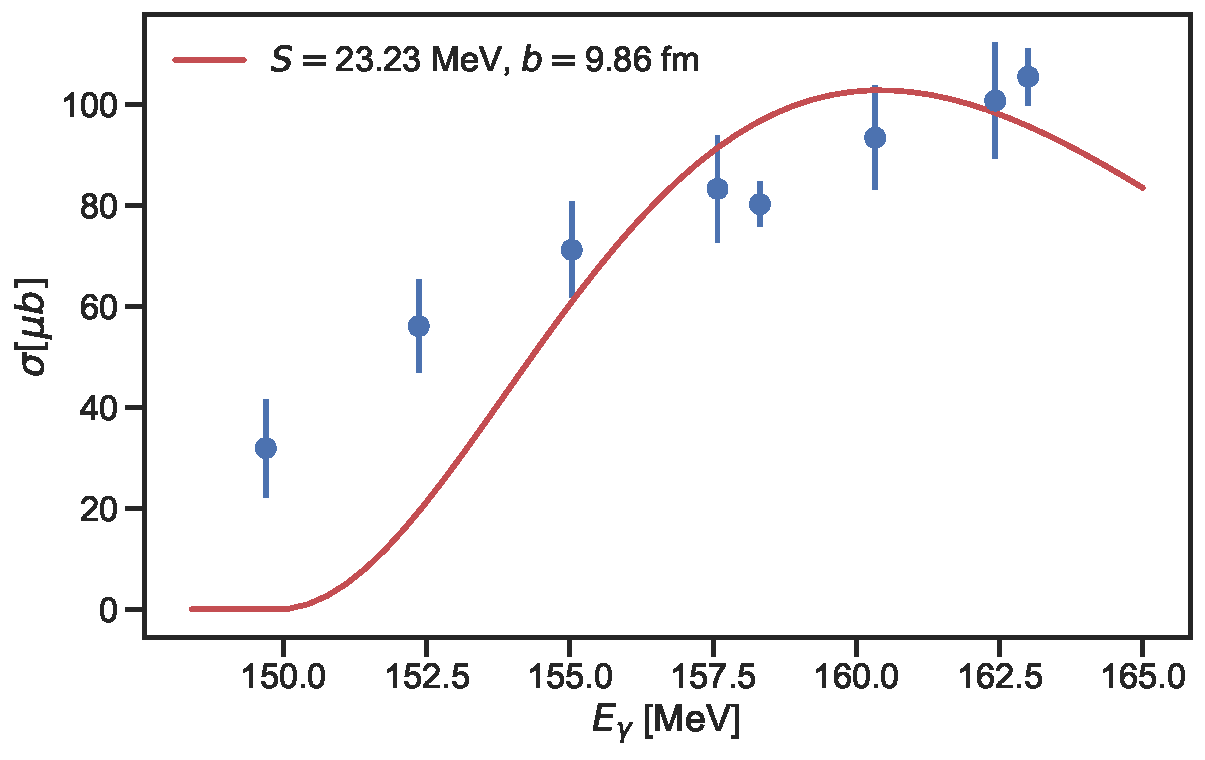
\includegraphics[width=\linewidth]{Figures/ChargedPionOffNeutron.pdf}
	\end{sidecaption}
\end{figure}
Figure \ref{fig:ChargedPionsOffNeutrons} shows a smaller range parameter $b$, which we would expect for two particles attracting each other. However, the model has some problems adequately describing the behaviour near the threshold. This might indicate that the one-pion approximation is insufficient, and one must include higher orders. Nonetheless, it is still possible to extract the relative weight of the $p\pi^-$ channel and the contribution to the mass of the dressed neutron. This is shown in figure \ref{fig:ContributionPlotMinus}
\begin{figure}[H]
	\begin{sidecaption}{Radial wave functions using the parameters shown in the figure. }[fig:ContributionPlotMinus]
		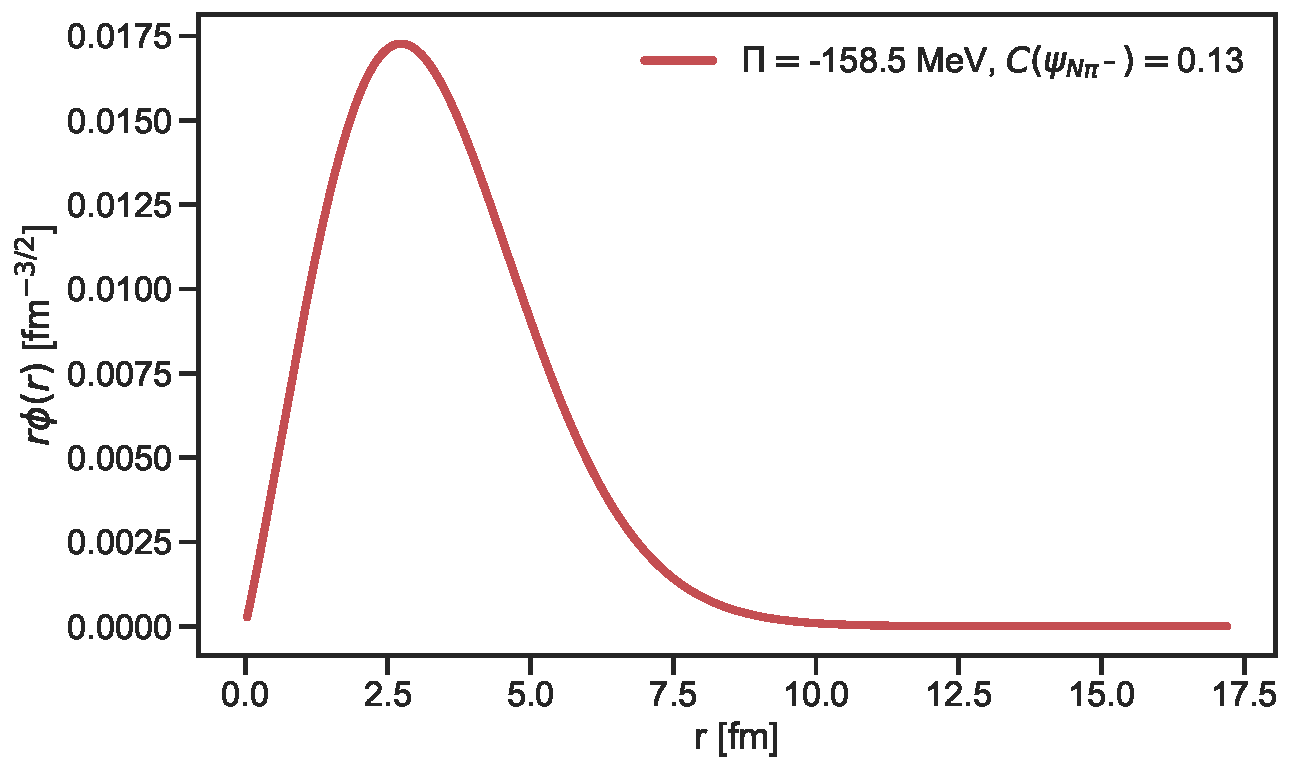
\includegraphics[width=\linewidth]{Figures/ContributionPlotPiMinus.pdf}
	\end{sidecaption}
\end{figure}
Since the strength parameter $S$ and the range parameter $b$ is smaller than the other processes, the contribution to the total wave function is also smaller. For the parameters shown in figure \ref{fig:ChargedPionsOffNeutrons} this is $0.13\%$. The contribution to the mass of the dressed neutron is also much smaller, only $-158.4$ MeV.

Following the same approach as in section \ref{sec:CoffP} we can calculate the charge density. Since we are considering a dressed neutron, the net charge must be 0. The charge density can be seen in figure \ref{fig:chargedensityminus}
\begin{figure}[H]
	\begin{sidecaption}{Charge density for the parameters $S=19.4$ MeV and $b=3.44$ fm. Note that the net charge is zero. }[fig:chargedensityminus]
		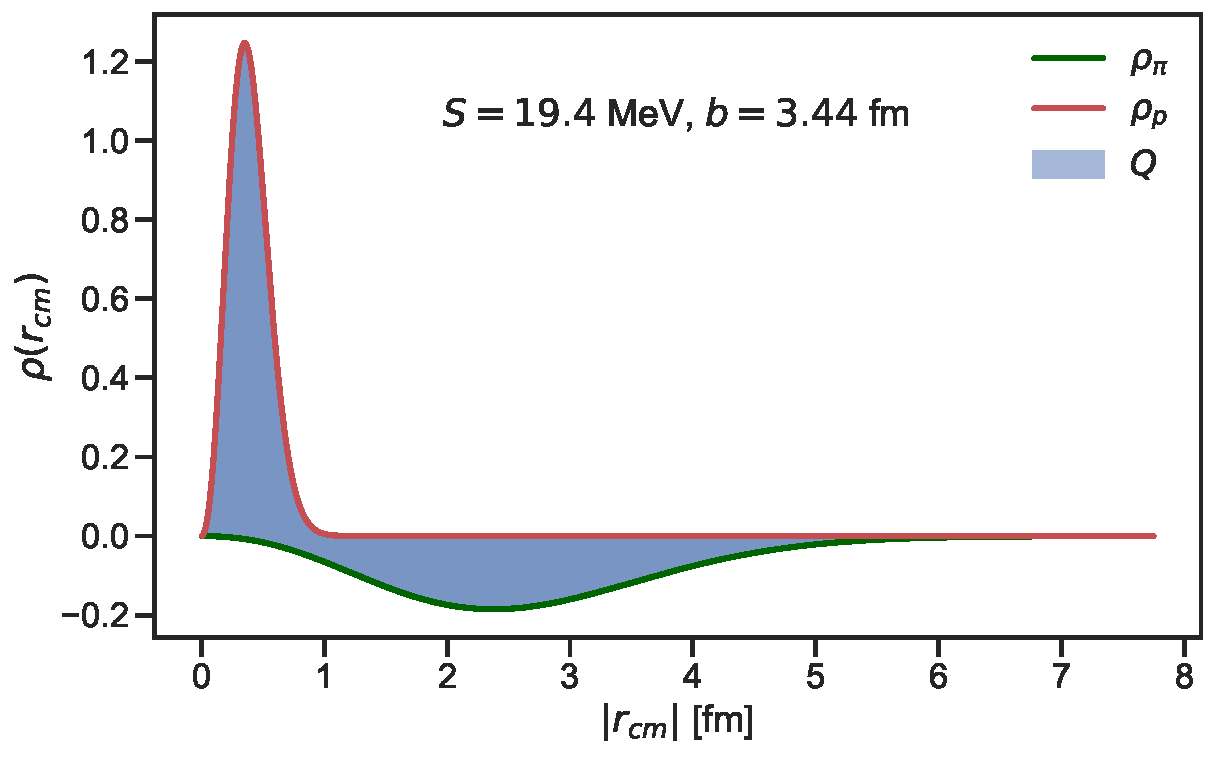
\includegraphics[width=\linewidth]{Figures/ChargeDensityNeutronMinus.pdf} 
	\end{sidecaption}
\end{figure}
This concludes the treatment of pion photoproduction of pions in the model with explicit pions.
\section{Discussion}\label{sec:discussion}
The expression for the total cross-section for neutral pion photoproduction off protons is shown in figure \ref{fig:crossfitrel} along with experimental data from \cite{Schmidt_2001}. The nuclear model with explicit pions can describe the behaviour of the total cross-section near the threshold when using the relativistic density of states. From figure \ref{fig:crossfitnonrel}, we see that relativistic effects become more important as the photon energy increases. By performing a fit, we can extract values for the strength parameter $S$ and the range parameter $b$. We found three sets of parameters able to describe the total cross-section within the framework of the model. To further test the validity of the parameters, we compared theoretical differential cross-section to experimental data from \cite{BeckPion}. Figure \ref{fig:MultipleEnergies} shows a decent agreement but also that the model has some trouble describing forward scattering. In particular, the agreement is much better for angles smaller than 90 degrees which can be investigated by inspecting equation \eqref{exactdiffcross}. The angular dependency originates from the sum over the polarisation index \eqref{sumoverpol} and the magnitude of the wave number vector \eqref{sexpanded}. Hence, the angular distribution is not a simple $\sin^2(\theta_q)$ as seen in figure \ref{fig:angular151}. An explanation could be that the one-pion approximation is not sufficient. For instance, the two-pion contributions change the wave number vector \eqref{sexpanded} in such a way that the integral $F(s)$ in equation \eqref{exactdiffcross} is much higher for larger angles. Quantitatively, this claim is supported by the results in figure \ref{fig:ContributionPlot}, where the contributions to the total wave function are shown. We see that the relative weight of the $\pi^0$ component in the wave function is within the range $24-29\%$. We expect the one-pion approximation to dominate near the threshold, but there will be a contribution from other components in the total multi-component wave function \eqref{superposition}. It is difficult to estimate the contributions without explicitly solving the new physical setup. This needs new considerations about how the dressing of the nucleon is done within the two-pion framework. As more pions enter the system, new numerical challenges are revealed as the approach used in chapter \ref{Decsofmodel} using coupled differential equations becomes more cumbersome as the number of particles increases. This can be circumvented by using a more general approach such as correlated Gaussians as in \cite{Fedorov2020}. 

Figure \ref{fig:neutralpionsoffneutrons} shows the total cross-section of the photoproduction of neutral pions off neutrons. Unfortunately, no experimental data exists near the threshold such that a fit can be performed. Once the experimental data is available, it is straightforward to use equation \eqref{pionneutraloffneutron}, and the parameters can be extracted. 

Figure \ref{fig:ChargedPionOffProton} shows the best fit of equation \eqref{totcross3} to experimental data from \cite{PionOffNeutron}. The model is able to describe the experimental data if one includes the contribution from the dipole approximation as seen in figure \ref{fig:CombinedPlot}. This leads to two sets of parameters describing the pion-nucleon system. For each set of parameters, we can estimate the charge density shown in figure \ref{fig:chargedensity} and figure \ref{fig:chargedensity1}. Ideally, the charge density of the pion-nucleon system would be a sum of figure \ref{fig:chargedensity} and figure \ref{fig:chargedensity1} since these two contributions constitute the total cross-section, but this brings new challenges in terms of normalisation since the net charge must be unity. 

Figure \ref{fig:ChargedPionsOffNeutrons} showed the fit of equation \eqref{totcross5} to experimental data. This is the most complicated process due to Coulomb interactions. This changes the dressing of the neutron where a three-component wave function is needed, and the final state is no longer a plane wave but a Coulomb wave. It is hard to specify what causes the fit to deviate so much from the others since Coulomb interactions are taken into account. As mentioned previously, the two-pion effects cannot be neglected even at the threshold. However, since the fit \ref{fig:ChargedPionsOffNeutrons} is considerably worse than the others, it might suggest something else need to be modified. This could be the form factor mentioned in section \ref{sec:formfactors} or an operator type of the form mentioned in section \ref{sec:EFT}.

\clearpage
\thispagestyle{empty}\mbox{}
\clearpage
